
% Default to the notebook output style

    


% Inherit from the specified cell style.




    
\documentclass[11pt]{article}

    
    
    \usepackage[T1]{fontenc}
    % Nicer default font (+ math font) than Computer Modern for most use cases
    \usepackage{mathpazo}

    % Basic figure setup, for now with no caption control since it's done
    % automatically by Pandoc (which extracts ![](path) syntax from Markdown).
    \usepackage{graphicx}
    % We will generate all images so they have a width \maxwidth. This means
    % that they will get their normal width if they fit onto the page, but
    % are scaled down if they would overflow the margins.
    \makeatletter
    \def\maxwidth{\ifdim\Gin@nat@width>\linewidth\linewidth
    \else\Gin@nat@width\fi}
    \makeatother
    \let\Oldincludegraphics\includegraphics
    % Set max figure width to be 80% of text width, for now hardcoded.
    \renewcommand{\includegraphics}[1]{\Oldincludegraphics[width=.8\maxwidth]{#1}}
    % Ensure that by default, figures have no caption (until we provide a
    % proper Figure object with a Caption API and a way to capture that
    % in the conversion process - todo).
    \usepackage{caption}
    \DeclareCaptionLabelFormat{nolabel}{}
    \captionsetup{labelformat=nolabel}

    \usepackage{adjustbox} % Used to constrain images to a maximum size 
    \usepackage{xcolor} % Allow colors to be defined
    \usepackage{enumerate} % Needed for markdown enumerations to work
    \usepackage{geometry} % Used to adjust the document margins
    \usepackage{amsmath} % Equations
    \usepackage{amssymb} % Equations
    \usepackage{textcomp} % defines textquotesingle
    % Hack from http://tex.stackexchange.com/a/47451/13684:
    \AtBeginDocument{%
        \def\PYZsq{\textquotesingle}% Upright quotes in Pygmentized code
    }
    \usepackage{upquote} % Upright quotes for verbatim code
    \usepackage{eurosym} % defines \euro
    \usepackage[mathletters]{ucs} % Extended unicode (utf-8) support
    \usepackage[utf8x]{inputenc} % Allow utf-8 characters in the tex document
    \usepackage{fancyvrb} % verbatim replacement that allows latex
    \usepackage{grffile} % extends the file name processing of package graphics 
                         % to support a larger range 
    % The hyperref package gives us a pdf with properly built
    % internal navigation ('pdf bookmarks' for the table of contents,
    % internal cross-reference links, web links for URLs, etc.)
    \usepackage{hyperref}
    \usepackage{longtable} % longtable support required by pandoc >1.10
    \usepackage{booktabs}  % table support for pandoc > 1.12.2
    \usepackage[inline]{enumitem} % IRkernel/repr support (it uses the enumerate* environment)
    \usepackage[normalem]{ulem} % ulem is needed to support strikethroughs (\sout)
                                % normalem makes italics be italics, not underlines
    

    \usepackage{float}
    
    % Colors for the hyperref package
    \definecolor{urlcolor}{rgb}{0,.145,.698}
    \definecolor{linkcolor}{rgb}{.71,0.21,0.01}
    \definecolor{citecolor}{rgb}{.12,.54,.11}

    % ANSI colors
    \definecolor{ansi-black}{HTML}{3E424D}
    \definecolor{ansi-black-intense}{HTML}{282C36}
    \definecolor{ansi-red}{HTML}{E75C58}
    \definecolor{ansi-red-intense}{HTML}{B22B31}
    \definecolor{ansi-green}{HTML}{00A250}
    \definecolor{ansi-green-intense}{HTML}{007427}
    \definecolor{ansi-yellow}{HTML}{DDB62B}
    \definecolor{ansi-yellow-intense}{HTML}{B27D12}
    \definecolor{ansi-blue}{HTML}{208FFB}
    \definecolor{ansi-blue-intense}{HTML}{0065CA}
    \definecolor{ansi-magenta}{HTML}{D160C4}
    \definecolor{ansi-magenta-intense}{HTML}{A03196}
    \definecolor{ansi-cyan}{HTML}{60C6C8}
    \definecolor{ansi-cyan-intense}{HTML}{258F8F}
    \definecolor{ansi-white}{HTML}{C5C1B4}
    \definecolor{ansi-white-intense}{HTML}{A1A6B2}

    % commands and environments needed by pandoc snippets
    % extracted from the output of `pandoc -s`
    \providecommand{\tightlist}{%
      \setlength{\itemsep}{0pt}\setlength{\parskip}{0pt}}
    \DefineVerbatimEnvironment{Highlighting}{Verbatim}{commandchars=\\\{\}}
    % Add ',fontsize=\small' for more characters per line
    \newenvironment{Shaded}{}{}
    \newcommand{\KeywordTok}[1]{\textcolor[rgb]{0.00,0.44,0.13}{\textbf{{#1}}}}
    \newcommand{\DataTypeTok}[1]{\textcolor[rgb]{0.56,0.13,0.00}{{#1}}}
    \newcommand{\DecValTok}[1]{\textcolor[rgb]{0.25,0.63,0.44}{{#1}}}
    \newcommand{\BaseNTok}[1]{\textcolor[rgb]{0.25,0.63,0.44}{{#1}}}
    \newcommand{\FloatTok}[1]{\textcolor[rgb]{0.25,0.63,0.44}{{#1}}}
    \newcommand{\CharTok}[1]{\textcolor[rgb]{0.25,0.44,0.63}{{#1}}}
    \newcommand{\StringTok}[1]{\textcolor[rgb]{0.25,0.44,0.63}{{#1}}}
    \newcommand{\CommentTok}[1]{\textcolor[rgb]{0.38,0.63,0.69}{\textit{{#1}}}}
    \newcommand{\OtherTok}[1]{\textcolor[rgb]{0.00,0.44,0.13}{{#1}}}
    \newcommand{\AlertTok}[1]{\textcolor[rgb]{1.00,0.00,0.00}{\textbf{{#1}}}}
    \newcommand{\FunctionTok}[1]{\textcolor[rgb]{0.02,0.16,0.49}{{#1}}}
    \newcommand{\RegionMarkerTok}[1]{{#1}}
    \newcommand{\ErrorTok}[1]{\textcolor[rgb]{1.00,0.00,0.00}{\textbf{{#1}}}}
    \newcommand{\NormalTok}[1]{{#1}}
    
    % Additional commands for more recent versions of Pandoc
    \newcommand{\ConstantTok}[1]{\textcolor[rgb]{0.53,0.00,0.00}{{#1}}}
    \newcommand{\SpecialCharTok}[1]{\textcolor[rgb]{0.25,0.44,0.63}{{#1}}}
    \newcommand{\VerbatimStringTok}[1]{\textcolor[rgb]{0.25,0.44,0.63}{{#1}}}
    \newcommand{\SpecialStringTok}[1]{\textcolor[rgb]{0.73,0.40,0.53}{{#1}}}
    \newcommand{\ImportTok}[1]{{#1}}
    \newcommand{\DocumentationTok}[1]{\textcolor[rgb]{0.73,0.13,0.13}{\textit{{#1}}}}
    \newcommand{\AnnotationTok}[1]{\textcolor[rgb]{0.38,0.63,0.69}{\textbf{\textit{{#1}}}}}
    \newcommand{\CommentVarTok}[1]{\textcolor[rgb]{0.38,0.63,0.69}{\textbf{\textit{{#1}}}}}
    \newcommand{\VariableTok}[1]{\textcolor[rgb]{0.10,0.09,0.49}{{#1}}}
    \newcommand{\ControlFlowTok}[1]{\textcolor[rgb]{0.00,0.44,0.13}{\textbf{{#1}}}}
    \newcommand{\OperatorTok}[1]{\textcolor[rgb]{0.40,0.40,0.40}{{#1}}}
    \newcommand{\BuiltInTok}[1]{{#1}}
    \newcommand{\ExtensionTok}[1]{{#1}}
    \newcommand{\PreprocessorTok}[1]{\textcolor[rgb]{0.74,0.48,0.00}{{#1}}}
    \newcommand{\AttributeTok}[1]{\textcolor[rgb]{0.49,0.56,0.16}{{#1}}}
    \newcommand{\InformationTok}[1]{\textcolor[rgb]{0.38,0.63,0.69}{\textbf{\textit{{#1}}}}}
    \newcommand{\WarningTok}[1]{\textcolor[rgb]{0.38,0.63,0.69}{\textbf{\textit{{#1}}}}}
    
    
    % Define a nice break command that doesn't care if a line doesn't already
    % exist.
    \def\br{\hspace*{\fill} \\* }
    % Math Jax compatability definitions
    \def\gt{>}
    \def\lt{<}
    % Document parameters
    \title{Probability Analysis of Monopoly}
    \author{L. Rotgers (larsrotgers@gmail.com)}
    
    
    

    % Pygments definitions
    
\makeatletter
\def\PY@reset{\let\PY@it=\relax \let\PY@bf=\relax%
    \let\PY@ul=\relax \let\PY@tc=\relax%
    \let\PY@bc=\relax \let\PY@ff=\relax}
\def\PY@tok#1{\csname PY@tok@#1\endcsname}
\def\PY@toks#1+{\ifx\relax#1\empty\else%
    \PY@tok{#1}\expandafter\PY@toks\fi}
\def\PY@do#1{\PY@bc{\PY@tc{\PY@ul{%
    \PY@it{\PY@bf{\PY@ff{#1}}}}}}}
\def\PY#1#2{\PY@reset\PY@toks#1+\relax+\PY@do{#2}}

\expandafter\def\csname PY@tok@w\endcsname{\def\PY@tc##1{\textcolor[rgb]{0.73,0.73,0.73}{##1}}}
\expandafter\def\csname PY@tok@c\endcsname{\let\PY@it=\textit\def\PY@tc##1{\textcolor[rgb]{0.25,0.50,0.50}{##1}}}
\expandafter\def\csname PY@tok@cp\endcsname{\def\PY@tc##1{\textcolor[rgb]{0.74,0.48,0.00}{##1}}}
\expandafter\def\csname PY@tok@k\endcsname{\let\PY@bf=\textbf\def\PY@tc##1{\textcolor[rgb]{0.00,0.50,0.00}{##1}}}
\expandafter\def\csname PY@tok@kp\endcsname{\def\PY@tc##1{\textcolor[rgb]{0.00,0.50,0.00}{##1}}}
\expandafter\def\csname PY@tok@kt\endcsname{\def\PY@tc##1{\textcolor[rgb]{0.69,0.00,0.25}{##1}}}
\expandafter\def\csname PY@tok@o\endcsname{\def\PY@tc##1{\textcolor[rgb]{0.40,0.40,0.40}{##1}}}
\expandafter\def\csname PY@tok@ow\endcsname{\let\PY@bf=\textbf\def\PY@tc##1{\textcolor[rgb]{0.67,0.13,1.00}{##1}}}
\expandafter\def\csname PY@tok@nb\endcsname{\def\PY@tc##1{\textcolor[rgb]{0.00,0.50,0.00}{##1}}}
\expandafter\def\csname PY@tok@nf\endcsname{\def\PY@tc##1{\textcolor[rgb]{0.00,0.00,1.00}{##1}}}
\expandafter\def\csname PY@tok@nc\endcsname{\let\PY@bf=\textbf\def\PY@tc##1{\textcolor[rgb]{0.00,0.00,1.00}{##1}}}
\expandafter\def\csname PY@tok@nn\endcsname{\let\PY@bf=\textbf\def\PY@tc##1{\textcolor[rgb]{0.00,0.00,1.00}{##1}}}
\expandafter\def\csname PY@tok@ne\endcsname{\let\PY@bf=\textbf\def\PY@tc##1{\textcolor[rgb]{0.82,0.25,0.23}{##1}}}
\expandafter\def\csname PY@tok@nv\endcsname{\def\PY@tc##1{\textcolor[rgb]{0.10,0.09,0.49}{##1}}}
\expandafter\def\csname PY@tok@no\endcsname{\def\PY@tc##1{\textcolor[rgb]{0.53,0.00,0.00}{##1}}}
\expandafter\def\csname PY@tok@nl\endcsname{\def\PY@tc##1{\textcolor[rgb]{0.63,0.63,0.00}{##1}}}
\expandafter\def\csname PY@tok@ni\endcsname{\let\PY@bf=\textbf\def\PY@tc##1{\textcolor[rgb]{0.60,0.60,0.60}{##1}}}
\expandafter\def\csname PY@tok@na\endcsname{\def\PY@tc##1{\textcolor[rgb]{0.49,0.56,0.16}{##1}}}
\expandafter\def\csname PY@tok@nt\endcsname{\let\PY@bf=\textbf\def\PY@tc##1{\textcolor[rgb]{0.00,0.50,0.00}{##1}}}
\expandafter\def\csname PY@tok@nd\endcsname{\def\PY@tc##1{\textcolor[rgb]{0.67,0.13,1.00}{##1}}}
\expandafter\def\csname PY@tok@s\endcsname{\def\PY@tc##1{\textcolor[rgb]{0.73,0.13,0.13}{##1}}}
\expandafter\def\csname PY@tok@sd\endcsname{\let\PY@it=\textit\def\PY@tc##1{\textcolor[rgb]{0.73,0.13,0.13}{##1}}}
\expandafter\def\csname PY@tok@si\endcsname{\let\PY@bf=\textbf\def\PY@tc##1{\textcolor[rgb]{0.73,0.40,0.53}{##1}}}
\expandafter\def\csname PY@tok@se\endcsname{\let\PY@bf=\textbf\def\PY@tc##1{\textcolor[rgb]{0.73,0.40,0.13}{##1}}}
\expandafter\def\csname PY@tok@sr\endcsname{\def\PY@tc##1{\textcolor[rgb]{0.73,0.40,0.53}{##1}}}
\expandafter\def\csname PY@tok@ss\endcsname{\def\PY@tc##1{\textcolor[rgb]{0.10,0.09,0.49}{##1}}}
\expandafter\def\csname PY@tok@sx\endcsname{\def\PY@tc##1{\textcolor[rgb]{0.00,0.50,0.00}{##1}}}
\expandafter\def\csname PY@tok@m\endcsname{\def\PY@tc##1{\textcolor[rgb]{0.40,0.40,0.40}{##1}}}
\expandafter\def\csname PY@tok@gh\endcsname{\let\PY@bf=\textbf\def\PY@tc##1{\textcolor[rgb]{0.00,0.00,0.50}{##1}}}
\expandafter\def\csname PY@tok@gu\endcsname{\let\PY@bf=\textbf\def\PY@tc##1{\textcolor[rgb]{0.50,0.00,0.50}{##1}}}
\expandafter\def\csname PY@tok@gd\endcsname{\def\PY@tc##1{\textcolor[rgb]{0.63,0.00,0.00}{##1}}}
\expandafter\def\csname PY@tok@gi\endcsname{\def\PY@tc##1{\textcolor[rgb]{0.00,0.63,0.00}{##1}}}
\expandafter\def\csname PY@tok@gr\endcsname{\def\PY@tc##1{\textcolor[rgb]{1.00,0.00,0.00}{##1}}}
\expandafter\def\csname PY@tok@ge\endcsname{\let\PY@it=\textit}
\expandafter\def\csname PY@tok@gs\endcsname{\let\PY@bf=\textbf}
\expandafter\def\csname PY@tok@gp\endcsname{\let\PY@bf=\textbf\def\PY@tc##1{\textcolor[rgb]{0.00,0.00,0.50}{##1}}}
\expandafter\def\csname PY@tok@go\endcsname{\def\PY@tc##1{\textcolor[rgb]{0.53,0.53,0.53}{##1}}}
\expandafter\def\csname PY@tok@gt\endcsname{\def\PY@tc##1{\textcolor[rgb]{0.00,0.27,0.87}{##1}}}
\expandafter\def\csname PY@tok@err\endcsname{\def\PY@bc##1{\setlength{\fboxsep}{0pt}\fcolorbox[rgb]{1.00,0.00,0.00}{1,1,1}{\strut ##1}}}
\expandafter\def\csname PY@tok@kc\endcsname{\let\PY@bf=\textbf\def\PY@tc##1{\textcolor[rgb]{0.00,0.50,0.00}{##1}}}
\expandafter\def\csname PY@tok@kd\endcsname{\let\PY@bf=\textbf\def\PY@tc##1{\textcolor[rgb]{0.00,0.50,0.00}{##1}}}
\expandafter\def\csname PY@tok@kn\endcsname{\let\PY@bf=\textbf\def\PY@tc##1{\textcolor[rgb]{0.00,0.50,0.00}{##1}}}
\expandafter\def\csname PY@tok@kr\endcsname{\let\PY@bf=\textbf\def\PY@tc##1{\textcolor[rgb]{0.00,0.50,0.00}{##1}}}
\expandafter\def\csname PY@tok@bp\endcsname{\def\PY@tc##1{\textcolor[rgb]{0.00,0.50,0.00}{##1}}}
\expandafter\def\csname PY@tok@fm\endcsname{\def\PY@tc##1{\textcolor[rgb]{0.00,0.00,1.00}{##1}}}
\expandafter\def\csname PY@tok@vc\endcsname{\def\PY@tc##1{\textcolor[rgb]{0.10,0.09,0.49}{##1}}}
\expandafter\def\csname PY@tok@vg\endcsname{\def\PY@tc##1{\textcolor[rgb]{0.10,0.09,0.49}{##1}}}
\expandafter\def\csname PY@tok@vi\endcsname{\def\PY@tc##1{\textcolor[rgb]{0.10,0.09,0.49}{##1}}}
\expandafter\def\csname PY@tok@vm\endcsname{\def\PY@tc##1{\textcolor[rgb]{0.10,0.09,0.49}{##1}}}
\expandafter\def\csname PY@tok@sa\endcsname{\def\PY@tc##1{\textcolor[rgb]{0.73,0.13,0.13}{##1}}}
\expandafter\def\csname PY@tok@sb\endcsname{\def\PY@tc##1{\textcolor[rgb]{0.73,0.13,0.13}{##1}}}
\expandafter\def\csname PY@tok@sc\endcsname{\def\PY@tc##1{\textcolor[rgb]{0.73,0.13,0.13}{##1}}}
\expandafter\def\csname PY@tok@dl\endcsname{\def\PY@tc##1{\textcolor[rgb]{0.73,0.13,0.13}{##1}}}
\expandafter\def\csname PY@tok@s2\endcsname{\def\PY@tc##1{\textcolor[rgb]{0.73,0.13,0.13}{##1}}}
\expandafter\def\csname PY@tok@sh\endcsname{\def\PY@tc##1{\textcolor[rgb]{0.73,0.13,0.13}{##1}}}
\expandafter\def\csname PY@tok@s1\endcsname{\def\PY@tc##1{\textcolor[rgb]{0.73,0.13,0.13}{##1}}}
\expandafter\def\csname PY@tok@mb\endcsname{\def\PY@tc##1{\textcolor[rgb]{0.40,0.40,0.40}{##1}}}
\expandafter\def\csname PY@tok@mf\endcsname{\def\PY@tc##1{\textcolor[rgb]{0.40,0.40,0.40}{##1}}}
\expandafter\def\csname PY@tok@mh\endcsname{\def\PY@tc##1{\textcolor[rgb]{0.40,0.40,0.40}{##1}}}
\expandafter\def\csname PY@tok@mi\endcsname{\def\PY@tc##1{\textcolor[rgb]{0.40,0.40,0.40}{##1}}}
\expandafter\def\csname PY@tok@il\endcsname{\def\PY@tc##1{\textcolor[rgb]{0.40,0.40,0.40}{##1}}}
\expandafter\def\csname PY@tok@mo\endcsname{\def\PY@tc##1{\textcolor[rgb]{0.40,0.40,0.40}{##1}}}
\expandafter\def\csname PY@tok@ch\endcsname{\let\PY@it=\textit\def\PY@tc##1{\textcolor[rgb]{0.25,0.50,0.50}{##1}}}
\expandafter\def\csname PY@tok@cm\endcsname{\let\PY@it=\textit\def\PY@tc##1{\textcolor[rgb]{0.25,0.50,0.50}{##1}}}
\expandafter\def\csname PY@tok@cpf\endcsname{\let\PY@it=\textit\def\PY@tc##1{\textcolor[rgb]{0.25,0.50,0.50}{##1}}}
\expandafter\def\csname PY@tok@c1\endcsname{\let\PY@it=\textit\def\PY@tc##1{\textcolor[rgb]{0.25,0.50,0.50}{##1}}}
\expandafter\def\csname PY@tok@cs\endcsname{\let\PY@it=\textit\def\PY@tc##1{\textcolor[rgb]{0.25,0.50,0.50}{##1}}}

\def\PYZbs{\char`\\}
\def\PYZus{\char`\_}
\def\PYZob{\char`\{}
\def\PYZcb{\char`\}}
\def\PYZca{\char`\^}
\def\PYZam{\char`\&}
\def\PYZlt{\char`\<}
\def\PYZgt{\char`\>}
\def\PYZsh{\char`\#}
\def\PYZpc{\char`\%}
\def\PYZdl{\char`\$}
\def\PYZhy{\char`\-}
\def\PYZsq{\char`\'}
\def\PYZdq{\char`\"}
\def\PYZti{\char`\~}
% for compatibility with earlier versions
\def\PYZat{@}
\def\PYZlb{[}
\def\PYZrb{]}
\makeatother


    % Exact colors from NB
    \definecolor{incolor}{rgb}{0.0, 0.0, 0.5}
    \definecolor{outcolor}{rgb}{0.545, 0.0, 0.0}



    
    % Prevent overflowing lines due to hard-to-break entities
    \sloppy 
    % Setup hyperref package
    \hypersetup{
      breaklinks=true,  % so long urls are correctly broken across lines
      colorlinks=true,
      urlcolor=urlcolor,
      linkcolor=linkcolor,
      citecolor=citecolor,
      }
    % Slightly bigger margins than the latex defaults
    
    \geometry{verbose,tmargin=1in,bmargin=1in,lmargin=1in,rmargin=1in}
    
    

    \begin{document}
    
    
    \maketitle
    \newpage
    \tableofcontents
    \newpage
  

    \hypertarget{probability-analysis-of-monopoly}{%
\section{Probability Analysis of
Monopoly}\label{probability-analysis-of-monopoly}}

    In this document we are going to analyze the probabilities in Monopoly
to answer the question: which are the best houses to buy?

To answer this question we will create a simulated version of Monopoly
and determine the probabilities to land on each square. Then we
calculate the expected value for each square. The squares with the
highest expected values are the best squares to have.

    \begin{figure}[H]
\centering
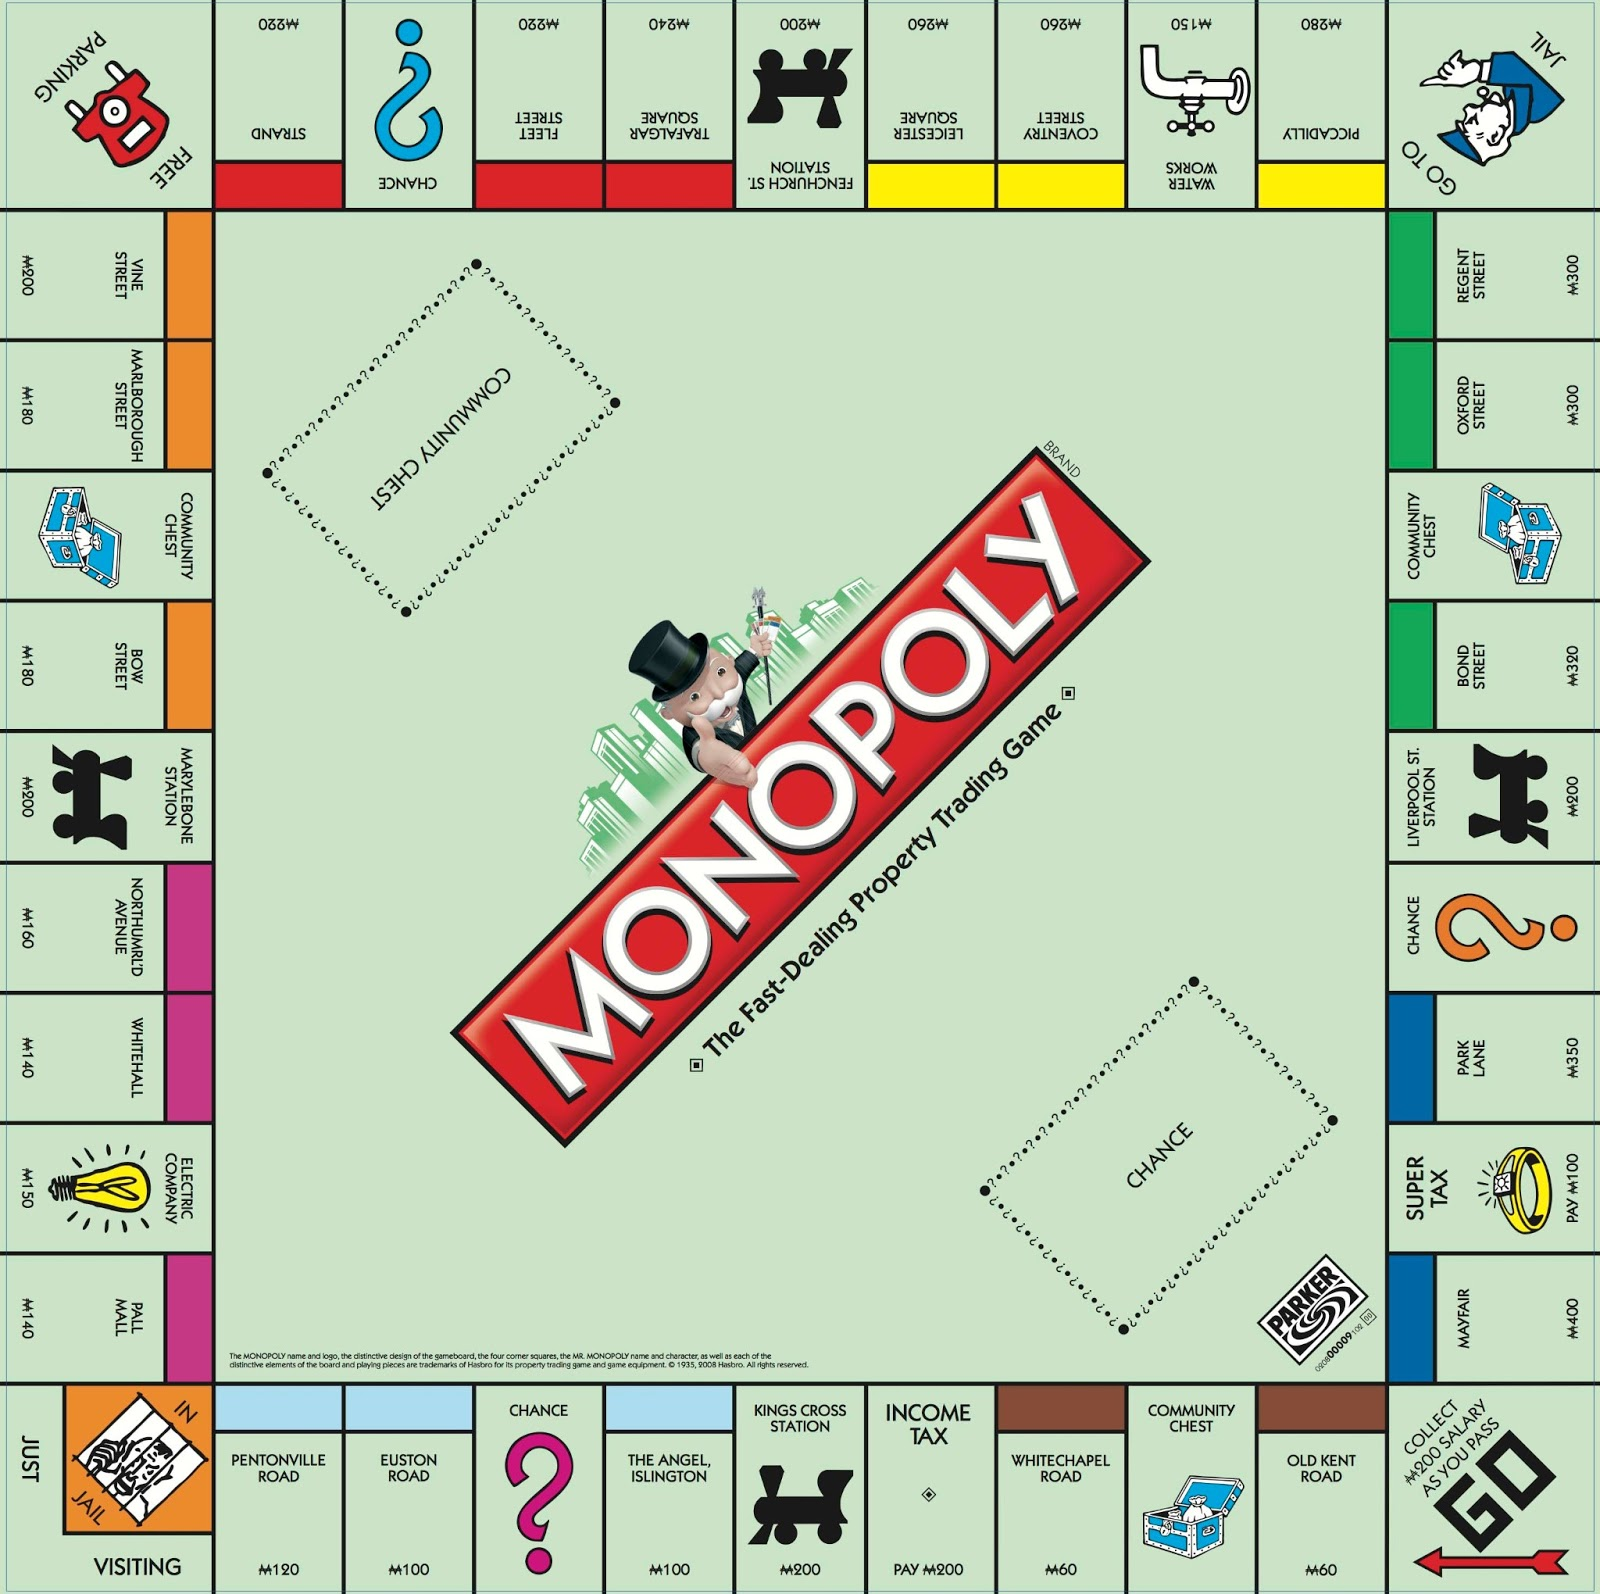
\includegraphics{monopoly_1.jpg}
\caption{monopoly}
\end{figure}

    \hypertarget{squares}{%
\subsection{Squares}\label{squares}}

    Each edge has 9 positions and there are 4 edges. There are 4 corners.
Which gives a total of 40 positions where a player can land. The labels
are numbered starting at GO.

    \hypertarget{labels}{%
\subsubsection{Labels}\label{labels}}

    \begin{Verbatim}[commandchars=\\\{\}]
{\color{incolor}In [{\color{incolor}2}]:} \PY{n}{squares\PYZus{}labels} \PY{o}{=} \PY{p}{[}\PY{l+s+s1}{\PYZsq{}}\PY{l+s+s1}{start}\PY{l+s+s1}{\PYZsq{}}\PY{p}{,} \PY{l+s+s1}{\PYZsq{}}\PY{l+s+s1}{b1}\PY{l+s+s1}{\PYZsq{}}\PY{p}{,} \PY{l+s+s1}{\PYZsq{}}\PY{l+s+s1}{cc1}\PY{l+s+s1}{\PYZsq{}}\PY{p}{,} \PY{l+s+s1}{\PYZsq{}}\PY{l+s+s1}{b2}\PY{l+s+s1}{\PYZsq{}}\PY{p}{,} \PY{l+s+s1}{\PYZsq{}}\PY{l+s+s1}{it}\PY{l+s+s1}{\PYZsq{}}\PY{p}{,} \PY{l+s+s1}{\PYZsq{}}\PY{l+s+s1}{t1}\PY{l+s+s1}{\PYZsq{}}\PY{p}{,} 
                          \PY{l+s+s1}{\PYZsq{}}\PY{l+s+s1}{lb1}\PY{l+s+s1}{\PYZsq{}}\PY{p}{,} \PY{l+s+s1}{\PYZsq{}}\PY{l+s+s1}{c1}\PY{l+s+s1}{\PYZsq{}}\PY{p}{,} \PY{l+s+s1}{\PYZsq{}}\PY{l+s+s1}{lb2}\PY{l+s+s1}{\PYZsq{}}\PY{p}{,} \PY{l+s+s1}{\PYZsq{}}\PY{l+s+s1}{lb3}\PY{l+s+s1}{\PYZsq{}}\PY{p}{,} \PY{l+s+s1}{\PYZsq{}}\PY{l+s+s1}{jail}\PY{l+s+s1}{\PYZsq{}}\PY{p}{,} \PY{l+s+s1}{\PYZsq{}}\PY{l+s+s1}{p1}\PY{l+s+s1}{\PYZsq{}}\PY{p}{,} 
                          \PY{l+s+s1}{\PYZsq{}}\PY{l+s+s1}{ec}\PY{l+s+s1}{\PYZsq{}}\PY{p}{,} \PY{l+s+s1}{\PYZsq{}}\PY{l+s+s1}{p2}\PY{l+s+s1}{\PYZsq{}}\PY{p}{,} \PY{l+s+s1}{\PYZsq{}}\PY{l+s+s1}{p3}\PY{l+s+s1}{\PYZsq{}}\PY{p}{,} \PY{l+s+s1}{\PYZsq{}}\PY{l+s+s1}{ts2}\PY{l+s+s1}{\PYZsq{}}\PY{p}{,} \PY{l+s+s1}{\PYZsq{}}\PY{l+s+s1}{o1}\PY{l+s+s1}{\PYZsq{}}\PY{p}{,} \PY{l+s+s1}{\PYZsq{}}\PY{l+s+s1}{cc2}\PY{l+s+s1}{\PYZsq{}}\PY{p}{,} 
                          \PY{l+s+s1}{\PYZsq{}}\PY{l+s+s1}{o2}\PY{l+s+s1}{\PYZsq{}}\PY{p}{,} \PY{l+s+s1}{\PYZsq{}}\PY{l+s+s1}{o3}\PY{l+s+s1}{\PYZsq{}}\PY{p}{,} \PY{l+s+s1}{\PYZsq{}}\PY{l+s+s1}{p}\PY{l+s+s1}{\PYZsq{}}\PY{p}{,} \PY{l+s+s1}{\PYZsq{}}\PY{l+s+s1}{r1}\PY{l+s+s1}{\PYZsq{}}\PY{p}{,} \PY{l+s+s1}{\PYZsq{}}\PY{l+s+s1}{c2}\PY{l+s+s1}{\PYZsq{}}\PY{p}{,} \PY{l+s+s1}{\PYZsq{}}\PY{l+s+s1}{r2}\PY{l+s+s1}{\PYZsq{}}\PY{p}{,} \PY{l+s+s1}{\PYZsq{}}\PY{l+s+s1}{r3}\PY{l+s+s1}{\PYZsq{}}\PY{p}{,} 
                          \PY{l+s+s1}{\PYZsq{}}\PY{l+s+s1}{ts3}\PY{l+s+s1}{\PYZsq{}}\PY{p}{,} \PY{l+s+s1}{\PYZsq{}}\PY{l+s+s1}{y1}\PY{l+s+s1}{\PYZsq{}}\PY{p}{,} \PY{l+s+s1}{\PYZsq{}}\PY{l+s+s1}{y2}\PY{l+s+s1}{\PYZsq{}}\PY{p}{,} \PY{l+s+s1}{\PYZsq{}}\PY{l+s+s1}{ww}\PY{l+s+s1}{\PYZsq{}}\PY{p}{,} \PY{l+s+s1}{\PYZsq{}}\PY{l+s+s1}{y3}\PY{l+s+s1}{\PYZsq{}}\PY{p}{,} \PY{l+s+s1}{\PYZsq{}}\PY{l+s+s1}{gtj}\PY{l+s+s1}{\PYZsq{}}\PY{p}{,} 
                          \PY{l+s+s1}{\PYZsq{}}\PY{l+s+s1}{g1}\PY{l+s+s1}{\PYZsq{}}\PY{p}{,} \PY{l+s+s1}{\PYZsq{}}\PY{l+s+s1}{g2}\PY{l+s+s1}{\PYZsq{}}\PY{p}{,} \PY{l+s+s1}{\PYZsq{}}\PY{l+s+s1}{cc3}\PY{l+s+s1}{\PYZsq{}}\PY{p}{,} \PY{l+s+s1}{\PYZsq{}}\PY{l+s+s1}{g3}\PY{l+s+s1}{\PYZsq{}}\PY{p}{,} \PY{l+s+s1}{\PYZsq{}}\PY{l+s+s1}{ts4}\PY{l+s+s1}{\PYZsq{}}\PY{p}{,} \PY{l+s+s1}{\PYZsq{}}\PY{l+s+s1}{c3}\PY{l+s+s1}{\PYZsq{}}\PY{p}{,} 
                          \PY{l+s+s1}{\PYZsq{}}\PY{l+s+s1}{db1}\PY{l+s+s1}{\PYZsq{}}\PY{p}{,} \PY{l+s+s1}{\PYZsq{}}\PY{l+s+s1}{st}\PY{l+s+s1}{\PYZsq{}}\PY{p}{,} \PY{l+s+s1}{\PYZsq{}}\PY{l+s+s1}{db2}\PY{l+s+s1}{\PYZsq{}}\PY{p}{]}
        
        \PY{n}{squares\PYZus{}total} \PY{o}{=} \PY{n+nb}{len}\PY{p}{(}\PY{n}{squares\PYZus{}labels}\PY{p}{)}
        \PY{n+nb}{print}\PY{p}{(}\PY{l+s+s1}{\PYZsq{}}\PY{l+s+s1}{There are }\PY{l+s+si}{\PYZob{}\PYZcb{}}\PY{l+s+s1}{ squares.}\PY{l+s+s1}{\PYZsq{}}\PY{o}{.}\PY{n}{format}\PY{p}{(}\PY{n}{squares\PYZus{}total}\PY{p}{)}\PY{p}{)}
\end{Verbatim}


    \begin{Verbatim}[commandchars=\\\{\}]
There are 40 squares.

    \end{Verbatim}

    \hypertarget{descriptions}{%
\subsubsection{Descriptions}\label{descriptions}}

    We also want to know the proper names, so we don't have to look up the
labels.

    \begin{Verbatim}[commandchars=\\\{\}]
{\color{incolor}In [{\color{incolor}3}]:} \PY{n}{squares\PYZus{}description} \PY{o}{=} \PY{p}{[}\PY{l+s+s1}{\PYZsq{}}\PY{l+s+s1}{Start}\PY{l+s+s1}{\PYZsq{}}\PY{p}{,} \PY{l+s+s1}{\PYZsq{}}\PY{l+s+s1}{Brown 1}\PY{l+s+s1}{\PYZsq{}}\PY{p}{,} \PY{l+s+s1}{\PYZsq{}}\PY{l+s+s1}{Community Chest 1}\PY{l+s+s1}{\PYZsq{}}\PY{p}{,} \PY{l+s+s1}{\PYZsq{}}\PY{l+s+s1}{Brown 2}\PY{l+s+s1}{\PYZsq{}}\PY{p}{,} 
                               \PY{l+s+s1}{\PYZsq{}}\PY{l+s+s1}{Income Tax}\PY{l+s+s1}{\PYZsq{}}\PY{p}{,} \PY{l+s+s1}{\PYZsq{}}\PY{l+s+s1}{Train Station 1}\PY{l+s+s1}{\PYZsq{}}\PY{p}{,} \PY{l+s+s1}{\PYZsq{}}\PY{l+s+s1}{Light Blue 1}\PY{l+s+s1}{\PYZsq{}}\PY{p}{,} 
                               \PY{l+s+s1}{\PYZsq{}}\PY{l+s+s1}{Chance 1}\PY{l+s+s1}{\PYZsq{}}\PY{p}{,} \PY{l+s+s1}{\PYZsq{}}\PY{l+s+s1}{Light Blue 2}\PY{l+s+s1}{\PYZsq{}}\PY{p}{,} \PY{l+s+s1}{\PYZsq{}}\PY{l+s+s1}{Light Blue 3}\PY{l+s+s1}{\PYZsq{}}\PY{p}{,} \PY{l+s+s1}{\PYZsq{}}\PY{l+s+s1}{Jail}\PY{l+s+s1}{\PYZsq{}}\PY{p}{,} 
                               \PY{l+s+s1}{\PYZsq{}}\PY{l+s+s1}{Purple 1}\PY{l+s+s1}{\PYZsq{}}\PY{p}{,} \PY{l+s+s1}{\PYZsq{}}\PY{l+s+s1}{Electric Company}\PY{l+s+s1}{\PYZsq{}}\PY{p}{,} \PY{l+s+s1}{\PYZsq{}}\PY{l+s+s1}{Purple 2}\PY{l+s+s1}{\PYZsq{}}\PY{p}{,} 
                               \PY{l+s+s1}{\PYZsq{}}\PY{l+s+s1}{Purple 3}\PY{l+s+s1}{\PYZsq{}}\PY{p}{,} \PY{l+s+s1}{\PYZsq{}}\PY{l+s+s1}{Train Station 2}\PY{l+s+s1}{\PYZsq{}}\PY{p}{,} \PY{l+s+s1}{\PYZsq{}}\PY{l+s+s1}{Orange 1}\PY{l+s+s1}{\PYZsq{}}\PY{p}{,} 
                               \PY{l+s+s1}{\PYZsq{}}\PY{l+s+s1}{Community Chest 2}\PY{l+s+s1}{\PYZsq{}}\PY{p}{,} \PY{l+s+s1}{\PYZsq{}}\PY{l+s+s1}{Orange 2}\PY{l+s+s1}{\PYZsq{}}\PY{p}{,} \PY{l+s+s1}{\PYZsq{}}\PY{l+s+s1}{Orange 3}\PY{l+s+s1}{\PYZsq{}}\PY{p}{,} 
                               \PY{l+s+s1}{\PYZsq{}}\PY{l+s+s1}{Free Parking}\PY{l+s+s1}{\PYZsq{}}\PY{p}{,} \PY{l+s+s1}{\PYZsq{}}\PY{l+s+s1}{Red 1}\PY{l+s+s1}{\PYZsq{}}\PY{p}{,} \PY{l+s+s1}{\PYZsq{}}\PY{l+s+s1}{Chance 2}\PY{l+s+s1}{\PYZsq{}}\PY{p}{,} \PY{l+s+s1}{\PYZsq{}}\PY{l+s+s1}{Red 2}\PY{l+s+s1}{\PYZsq{}}\PY{p}{,} 
                               \PY{l+s+s1}{\PYZsq{}}\PY{l+s+s1}{Red 3}\PY{l+s+s1}{\PYZsq{}}\PY{p}{,} \PY{l+s+s1}{\PYZsq{}}\PY{l+s+s1}{Train Station 3}\PY{l+s+s1}{\PYZsq{}}\PY{p}{,} \PY{l+s+s1}{\PYZsq{}}\PY{l+s+s1}{Yellow 1}\PY{l+s+s1}{\PYZsq{}}\PY{p}{,} \PY{l+s+s1}{\PYZsq{}}\PY{l+s+s1}{Yellow 2}\PY{l+s+s1}{\PYZsq{}}\PY{p}{,} 
                               \PY{l+s+s1}{\PYZsq{}}\PY{l+s+s1}{Water Works}\PY{l+s+s1}{\PYZsq{}}\PY{p}{,} \PY{l+s+s1}{\PYZsq{}}\PY{l+s+s1}{Yellow 3}\PY{l+s+s1}{\PYZsq{}}\PY{p}{,} \PY{l+s+s1}{\PYZsq{}}\PY{l+s+s1}{Go to Jail}\PY{l+s+s1}{\PYZsq{}}\PY{p}{,} \PY{l+s+s1}{\PYZsq{}}\PY{l+s+s1}{Green 1}\PY{l+s+s1}{\PYZsq{}}\PY{p}{,} 
                               \PY{l+s+s1}{\PYZsq{}}\PY{l+s+s1}{Green 2}\PY{l+s+s1}{\PYZsq{}}\PY{p}{,} \PY{l+s+s1}{\PYZsq{}}\PY{l+s+s1}{Community Chest 3}\PY{l+s+s1}{\PYZsq{}}\PY{p}{,} \PY{l+s+s1}{\PYZsq{}}\PY{l+s+s1}{Green 3}\PY{l+s+s1}{\PYZsq{}}\PY{p}{,} 
                               \PY{l+s+s1}{\PYZsq{}}\PY{l+s+s1}{Train Station 4}\PY{l+s+s1}{\PYZsq{}}\PY{p}{,} \PY{l+s+s1}{\PYZsq{}}\PY{l+s+s1}{Chance 3}\PY{l+s+s1}{\PYZsq{}}\PY{p}{,} \PY{l+s+s1}{\PYZsq{}}\PY{l+s+s1}{Dark Blue 1}\PY{l+s+s1}{\PYZsq{}}\PY{p}{,} 
                               \PY{l+s+s1}{\PYZsq{}}\PY{l+s+s1}{Super Tax}\PY{l+s+s1}{\PYZsq{}}\PY{p}{,} \PY{l+s+s1}{\PYZsq{}}\PY{l+s+s1}{Dark Blue 2}\PY{l+s+s1}{\PYZsq{}}\PY{p}{]}
\end{Verbatim}


    \begin{Verbatim}[commandchars=\\\{\}]
{\color{incolor}In [{\color{incolor}4}]:} \PY{n+nb}{print}\PY{p}{(}\PY{l+s+s1}{\PYZsq{}}\PY{l+s+s1}{There are }\PY{l+s+si}{\PYZob{}\PYZcb{}}\PY{l+s+s1}{ descriptions.}\PY{l+s+s1}{\PYZsq{}}\PY{o}{.}\PY{n}{format}\PY{p}{(}\PY{n+nb}{len}\PY{p}{(}\PY{n}{squares\PYZus{}description}\PY{p}{)}\PY{p}{)}\PY{p}{)}
\end{Verbatim}


    \begin{Verbatim}[commandchars=\\\{\}]
There are 40 descriptions.

    \end{Verbatim}

    \hypertarget{purchasable}{%
\subsubsection{Purchasable}\label{purchasable}}

    We want to know if they are purchasable so we can sort on that later.

    \begin{Verbatim}[commandchars=\\\{\}]
{\color{incolor}In [{\color{incolor}5}]:} \PY{n}{squares\PYZus{}purchasable} \PY{o}{=} \PY{p}{[}\PY{k+kc}{False}\PY{p}{,} \PY{k+kc}{True}\PY{p}{,} \PY{k+kc}{False}\PY{p}{,} \PY{k+kc}{True}\PY{p}{,} \PY{k+kc}{False}\PY{p}{,} 
                               \PY{k+kc}{True}\PY{p}{,} \PY{k+kc}{True}\PY{p}{,} \PY{k+kc}{False}\PY{p}{,} \PY{k+kc}{True}\PY{p}{,} \PY{k+kc}{True}\PY{p}{,} 
                               \PY{k+kc}{False}\PY{p}{,} \PY{k+kc}{True}\PY{p}{,} \PY{k+kc}{True}\PY{p}{,} \PY{k+kc}{True}\PY{p}{,} \PY{k+kc}{True}\PY{p}{,} 
                               \PY{k+kc}{True}\PY{p}{,} \PY{k+kc}{True}\PY{p}{,} \PY{k+kc}{False}\PY{p}{,} \PY{k+kc}{True}\PY{p}{,} \PY{k+kc}{True}\PY{p}{,} 
                               \PY{k+kc}{False}\PY{p}{,} \PY{k+kc}{True}\PY{p}{,} \PY{k+kc}{False}\PY{p}{,} \PY{k+kc}{True}\PY{p}{,} \PY{k+kc}{True}\PY{p}{,} 
                               \PY{k+kc}{True}\PY{p}{,} \PY{k+kc}{True}\PY{p}{,} \PY{k+kc}{True}\PY{p}{,} \PY{k+kc}{True}\PY{p}{,} \PY{k+kc}{True}\PY{p}{,} 
                               \PY{k+kc}{False}\PY{p}{,} \PY{k+kc}{True}\PY{p}{,} \PY{k+kc}{True}\PY{p}{,} \PY{k+kc}{False}\PY{p}{,} \PY{k+kc}{True}\PY{p}{,} 
                               \PY{k+kc}{True}\PY{p}{,} \PY{k+kc}{False}\PY{p}{,} \PY{k+kc}{True}\PY{p}{,} \PY{k+kc}{False}\PY{p}{,} \PY{k+kc}{True}\PY{p}{]}
\end{Verbatim}


    \hypertarget{rent}{%
\subsubsection{Rent}\label{rent}}

    We want to use the rent paid at each square to calculate the expected
value. The utility company charge \(4\) times roll if one is owned, and
\(10\) times roll if both owned. For one railway we charge \(25\), two
\(50\), three \(100\), and all four \(200\).

    To find the rent for a utility company, we find the expected value for
throwing a dices times \(4\).

\[ 4\cdot E(\bar{k}) = 4 \cdot \dfrac{1}{6} \cdot (1+2+3+4+5+6) \]

    \begin{Verbatim}[commandchars=\\\{\}]
{\color{incolor}In [{\color{incolor}6}]:} \PY{n}{E\PYZus{}u} \PY{o}{=} \PY{l+m+mi}{4} \PY{o}{*} \PY{p}{(}\PY{l+m+mi}{1}\PY{o}{+}\PY{l+m+mi}{2}\PY{o}{+}\PY{l+m+mi}{3}\PY{o}{+}\PY{l+m+mi}{4}\PY{o}{+}\PY{l+m+mi}{5}\PY{o}{+}\PY{l+m+mi}{6}\PY{p}{)} \PY{o}{/} \PY{l+m+mi}{6}
\end{Verbatim}


    We pick the value for one railway which is \(25\).

    \begin{Verbatim}[commandchars=\\\{\}]
{\color{incolor}In [{\color{incolor}7}]:} \PY{n}{E\PYZus{}r} \PY{o}{=} \PY{l+m+mi}{25}
\end{Verbatim}


    \begin{Verbatim}[commandchars=\\\{\}]
{\color{incolor}In [{\color{incolor}8}]:} \PY{n}{squares\PYZus{}rent} \PY{o}{=} \PY{p}{[}\PY{l+m+mi}{0}\PY{p}{,} \PY{l+m+mi}{2}\PY{p}{,} \PY{l+m+mi}{0}\PY{p}{,} \PY{l+m+mi}{4}\PY{p}{,} \PY{l+m+mi}{0}\PY{p}{,} \PY{n}{E\PYZus{}r}\PY{p}{,} \PY{l+m+mi}{6}\PY{p}{,} \PY{l+m+mi}{0}\PY{p}{,} \PY{l+m+mi}{6}\PY{p}{,} \PY{l+m+mi}{8}\PY{p}{,} \PY{l+m+mi}{0}\PY{p}{,} \PY{l+m+mi}{10}\PY{p}{,} \PY{n}{E\PYZus{}u}\PY{p}{,} 
                        \PY{l+m+mi}{10}\PY{p}{,} \PY{l+m+mi}{12}\PY{p}{,} \PY{n}{E\PYZus{}r}\PY{p}{,} \PY{l+m+mi}{14}\PY{p}{,} \PY{l+m+mi}{0}\PY{p}{,} \PY{l+m+mi}{14}\PY{p}{,} \PY{l+m+mi}{16}\PY{p}{,} \PY{l+m+mi}{0}\PY{p}{,} \PY{l+m+mi}{18}\PY{p}{,} \PY{l+m+mi}{0}\PY{p}{,} \PY{l+m+mi}{18}\PY{p}{,} 
                        \PY{l+m+mi}{20}\PY{p}{,} \PY{n}{E\PYZus{}r}\PY{p}{,} \PY{l+m+mi}{22}\PY{p}{,} \PY{l+m+mi}{22}\PY{p}{,} \PY{n}{E\PYZus{}u}\PY{p}{,} \PY{l+m+mi}{24}\PY{p}{,} \PY{l+m+mi}{0}\PY{p}{,} \PY{l+m+mi}{26}\PY{p}{,} \PY{l+m+mi}{26}\PY{p}{,} \PY{l+m+mi}{0}\PY{p}{,} \PY{l+m+mi}{28}\PY{p}{,} 
                        \PY{n}{E\PYZus{}r}\PY{p}{,} \PY{l+m+mi}{0}\PY{p}{,} \PY{l+m+mi}{35}\PY{p}{,} \PY{l+m+mi}{0}\PY{p}{,} \PY{l+m+mi}{50}\PY{p}{]}
\end{Verbatim}


    \hypertarget{grouping}{%
\subsubsection{Grouping}\label{grouping}}

    We want to know in what group they are so we can aggregate our data
later.

    \begin{Verbatim}[commandchars=\\\{\}]
{\color{incolor}In [{\color{incolor}9}]:} \PY{n}{squares\PYZus{}aggregate} \PY{o}{=} \PY{p}{[}\PY{l+s+s1}{\PYZsq{}}\PY{l+s+s1}{Start}\PY{l+s+s1}{\PYZsq{}}\PY{p}{,} \PY{l+s+s1}{\PYZsq{}}\PY{l+s+s1}{Brown}\PY{l+s+s1}{\PYZsq{}}\PY{p}{,} \PY{l+s+s1}{\PYZsq{}}\PY{l+s+s1}{Community Chest}\PY{l+s+s1}{\PYZsq{}}\PY{p}{,} \PY{l+s+s1}{\PYZsq{}}\PY{l+s+s1}{Brown}\PY{l+s+s1}{\PYZsq{}}\PY{p}{,} 
                             \PY{l+s+s1}{\PYZsq{}}\PY{l+s+s1}{Income Tax}\PY{l+s+s1}{\PYZsq{}}\PY{p}{,} \PY{l+s+s1}{\PYZsq{}}\PY{l+s+s1}{Train Station}\PY{l+s+s1}{\PYZsq{}}\PY{p}{,} \PY{l+s+s1}{\PYZsq{}}\PY{l+s+s1}{Light Blue}\PY{l+s+s1}{\PYZsq{}}\PY{p}{,} 
                             \PY{l+s+s1}{\PYZsq{}}\PY{l+s+s1}{Chance}\PY{l+s+s1}{\PYZsq{}}\PY{p}{,} \PY{l+s+s1}{\PYZsq{}}\PY{l+s+s1}{Light Blue}\PY{l+s+s1}{\PYZsq{}}\PY{p}{,} \PY{l+s+s1}{\PYZsq{}}\PY{l+s+s1}{Light Blue}\PY{l+s+s1}{\PYZsq{}}\PY{p}{,} \PY{l+s+s1}{\PYZsq{}}\PY{l+s+s1}{Jail}\PY{l+s+s1}{\PYZsq{}}\PY{p}{,} 
                             \PY{l+s+s1}{\PYZsq{}}\PY{l+s+s1}{Purple}\PY{l+s+s1}{\PYZsq{}}\PY{p}{,} \PY{l+s+s1}{\PYZsq{}}\PY{l+s+s1}{Utilities}\PY{l+s+s1}{\PYZsq{}}\PY{p}{,} \PY{l+s+s1}{\PYZsq{}}\PY{l+s+s1}{Purple}\PY{l+s+s1}{\PYZsq{}}\PY{p}{,} \PY{l+s+s1}{\PYZsq{}}\PY{l+s+s1}{Purple}\PY{l+s+s1}{\PYZsq{}}\PY{p}{,} 
                             \PY{l+s+s1}{\PYZsq{}}\PY{l+s+s1}{Train Station}\PY{l+s+s1}{\PYZsq{}}\PY{p}{,} \PY{l+s+s1}{\PYZsq{}}\PY{l+s+s1}{Orange}\PY{l+s+s1}{\PYZsq{}}\PY{p}{,} \PY{l+s+s1}{\PYZsq{}}\PY{l+s+s1}{Community Chest}\PY{l+s+s1}{\PYZsq{}}\PY{p}{,} 
                             \PY{l+s+s1}{\PYZsq{}}\PY{l+s+s1}{Orange}\PY{l+s+s1}{\PYZsq{}}\PY{p}{,} \PY{l+s+s1}{\PYZsq{}}\PY{l+s+s1}{Orange}\PY{l+s+s1}{\PYZsq{}}\PY{p}{,} \PY{l+s+s1}{\PYZsq{}}\PY{l+s+s1}{Free Parking}\PY{l+s+s1}{\PYZsq{}}\PY{p}{,} \PY{l+s+s1}{\PYZsq{}}\PY{l+s+s1}{Red}\PY{l+s+s1}{\PYZsq{}}\PY{p}{,} 
                             \PY{l+s+s1}{\PYZsq{}}\PY{l+s+s1}{Chance}\PY{l+s+s1}{\PYZsq{}}\PY{p}{,} \PY{l+s+s1}{\PYZsq{}}\PY{l+s+s1}{Red}\PY{l+s+s1}{\PYZsq{}}\PY{p}{,} \PY{l+s+s1}{\PYZsq{}}\PY{l+s+s1}{Red}\PY{l+s+s1}{\PYZsq{}}\PY{p}{,} \PY{l+s+s1}{\PYZsq{}}\PY{l+s+s1}{Train Station}\PY{l+s+s1}{\PYZsq{}}\PY{p}{,} \PY{l+s+s1}{\PYZsq{}}\PY{l+s+s1}{Yellow}\PY{l+s+s1}{\PYZsq{}}\PY{p}{,} 
                             \PY{l+s+s1}{\PYZsq{}}\PY{l+s+s1}{Yellow}\PY{l+s+s1}{\PYZsq{}}\PY{p}{,} \PY{l+s+s1}{\PYZsq{}}\PY{l+s+s1}{Utilities}\PY{l+s+s1}{\PYZsq{}}\PY{p}{,} \PY{l+s+s1}{\PYZsq{}}\PY{l+s+s1}{Yellow}\PY{l+s+s1}{\PYZsq{}}\PY{p}{,} \PY{l+s+s1}{\PYZsq{}}\PY{l+s+s1}{Go to Jail}\PY{l+s+s1}{\PYZsq{}}\PY{p}{,} 
                             \PY{l+s+s1}{\PYZsq{}}\PY{l+s+s1}{Green}\PY{l+s+s1}{\PYZsq{}}\PY{p}{,} \PY{l+s+s1}{\PYZsq{}}\PY{l+s+s1}{Green}\PY{l+s+s1}{\PYZsq{}}\PY{p}{,} \PY{l+s+s1}{\PYZsq{}}\PY{l+s+s1}{Community Chest}\PY{l+s+s1}{\PYZsq{}}\PY{p}{,} \PY{l+s+s1}{\PYZsq{}}\PY{l+s+s1}{Green}\PY{l+s+s1}{\PYZsq{}}\PY{p}{,} 
                             \PY{l+s+s1}{\PYZsq{}}\PY{l+s+s1}{Train Station}\PY{l+s+s1}{\PYZsq{}}\PY{p}{,} \PY{l+s+s1}{\PYZsq{}}\PY{l+s+s1}{Chance}\PY{l+s+s1}{\PYZsq{}}\PY{p}{,} \PY{l+s+s1}{\PYZsq{}}\PY{l+s+s1}{Dark Blue}\PY{l+s+s1}{\PYZsq{}}\PY{p}{,} 
                             \PY{l+s+s1}{\PYZsq{}}\PY{l+s+s1}{Super Tax}\PY{l+s+s1}{\PYZsq{}}\PY{p}{,} \PY{l+s+s1}{\PYZsq{}}\PY{l+s+s1}{Dark Blue}\PY{l+s+s1}{\PYZsq{}}\PY{p}{]}
\end{Verbatim}


    \hypertarget{cards}{%
\subsection{Cards}\label{cards}}

    There are two decks of cards.

\begin{itemize}
\tightlist
\item
  Community Cards
\item
  Chance Cards
\end{itemize}

Each deck contains 16 cards.

    \hypertarget{community-cards}{%
\subsubsection{Community Cards}\label{community-cards}}

    Monopoly has \(16\) community cards.

    \begin{figure}[H]
\centering
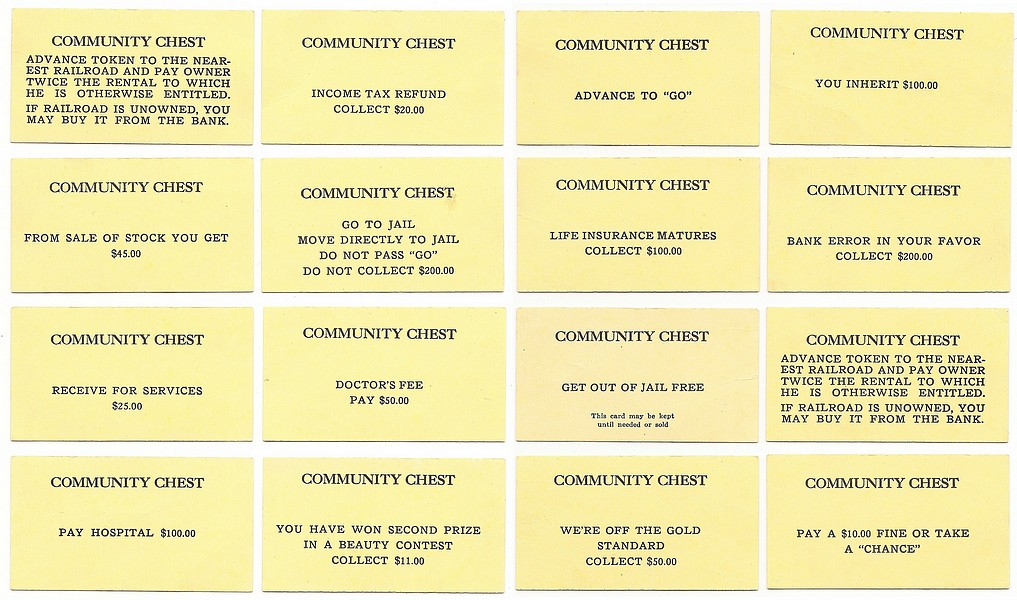
\includegraphics{monopoly_2.jpg}
\caption{cc}
\end{figure}

    Because we are only determining the probabilities, we are only
interested in the following cards:

\begin{itemize}
\tightlist
\item
  advance to go
\item
  go to jail
\item
  get out of jail, free
\item
  go back 2 spaces
\end{itemize}

    \hypertarget{community-deck-implementation}{%
\subsubsection{Community deck
implementation}\label{community-deck-implementation}}

    We implement the community deck in a class. The class keeps track of a
list with \(16\) cards. An index points to the next card. When we are
out of cards, we reset the index and reshuffle the cards.

    \begin{Verbatim}[commandchars=\\\{\}]
{\color{incolor}In [{\color{incolor}10}]:} \PY{k+kn}{from} \PY{n+nn}{random} \PY{k}{import} \PY{n}{shuffle}
         
         \PY{k}{class} \PY{n+nc}{CommunityDeck}\PY{p}{(}\PY{p}{)}\PY{p}{:}
             \PY{k}{def} \PY{n+nf}{\PYZus{}\PYZus{}init\PYZus{}\PYZus{}}\PY{p}{(}\PY{n+nb+bp}{self}\PY{p}{)}\PY{p}{:}
                 \PY{n+nb+bp}{self}\PY{o}{.}\PY{n}{deck} \PY{o}{=} \PY{p}{[}\PY{l+m+mi}{0}\PY{p}{]} \PY{o}{*} \PY{l+m+mi}{16}
                 \PY{n+nb+bp}{self}\PY{o}{.}\PY{n}{deck}\PY{p}{[}\PY{l+m+mi}{0}\PY{p}{]} \PY{o}{=} \PY{l+s+s1}{\PYZsq{}}\PY{l+s+s1}{gtg}\PY{l+s+s1}{\PYZsq{}} \PY{c+c1}{\PYZsh{} go to go}
                 \PY{n+nb+bp}{self}\PY{o}{.}\PY{n}{deck}\PY{p}{[}\PY{l+m+mi}{1}\PY{p}{]} \PY{o}{=} \PY{l+s+s1}{\PYZsq{}}\PY{l+s+s1}{gtj}\PY{l+s+s1}{\PYZsq{}} \PY{c+c1}{\PYZsh{} go to jail}
                 \PY{n+nb+bp}{self}\PY{o}{.}\PY{n}{deck}\PY{p}{[}\PY{l+m+mi}{2}\PY{p}{]} \PY{o}{=} \PY{l+s+s1}{\PYZsq{}}\PY{l+s+s1}{goj}\PY{l+s+s1}{\PYZsq{}} \PY{c+c1}{\PYZsh{} get out of jail }
                 \PY{n+nb+bp}{self}\PY{o}{.}\PY{n}{deck}\PY{p}{[}\PY{l+m+mi}{3}\PY{p}{]} \PY{o}{=} \PY{l+s+s1}{\PYZsq{}}\PY{l+s+s1}{gb2}\PY{l+s+s1}{\PYZsq{}} \PY{c+c1}{\PYZsh{} go back 2 steps}
                 \PY{n+nb+bp}{self}\PY{o}{.}\PY{n}{index} \PY{o}{=} \PY{l+m+mi}{16}
             
             \PY{k}{def} \PY{n+nf}{draw\PYZus{}card}\PY{p}{(}\PY{n+nb+bp}{self}\PY{p}{)}\PY{p}{:}
                 \PY{k}{if} \PY{n+nb+bp}{self}\PY{o}{.}\PY{n}{index} \PY{o}{\PYZgt{}}\PY{o}{=} \PY{n+nb}{len}\PY{p}{(}\PY{n+nb+bp}{self}\PY{o}{.}\PY{n}{deck}\PY{p}{)}\PY{p}{:}
                     \PY{n+nb+bp}{self}\PY{o}{.}\PY{n}{index} \PY{o}{=} \PY{l+m+mi}{0}
                     \PY{n}{shuffle}\PY{p}{(}\PY{n+nb+bp}{self}\PY{o}{.}\PY{n}{deck}\PY{p}{)}
                 \PY{n}{card} \PY{o}{=} \PY{n+nb+bp}{self}\PY{o}{.}\PY{n}{deck}\PY{p}{[}\PY{n+nb+bp}{self}\PY{o}{.}\PY{n}{index}\PY{p}{]}
                 \PY{n+nb+bp}{self}\PY{o}{.}\PY{n}{index} \PY{o}{+}\PY{o}{=} \PY{l+m+mi}{1}
                 \PY{k}{return} \PY{n}{card}
\end{Verbatim}


    Now we test it:

    \begin{Verbatim}[commandchars=\\\{\}]
{\color{incolor}In [{\color{incolor}11}]:} \PY{n}{deck} \PY{o}{=} \PY{n}{CommunityDeck}\PY{p}{(}\PY{p}{)}
         \PY{n}{deck}\PY{o}{.}\PY{n}{deck}
\end{Verbatim}


\begin{Verbatim}[commandchars=\\\{\}]
{\color{outcolor}Out[{\color{outcolor}11}]:} ['gtg', 'gtj', 'goj', 'gb2', 0, 0, 0, 0, 0, 0, 0, 0, 0, 0, 0, 0]
\end{Verbatim}
            
    \begin{Verbatim}[commandchars=\\\{\}]
{\color{incolor}In [{\color{incolor}12}]:} \PY{n}{deck}\PY{o}{.}\PY{n}{draw\PYZus{}card}\PY{p}{(}\PY{p}{)}
\end{Verbatim}


\begin{Verbatim}[commandchars=\\\{\}]
{\color{outcolor}Out[{\color{outcolor}12}]:} 0
\end{Verbatim}
            
    \begin{Verbatim}[commandchars=\\\{\}]
{\color{incolor}In [{\color{incolor}13}]:} \PY{n}{deck}\PY{o}{.}\PY{n}{deck}
\end{Verbatim}


\begin{Verbatim}[commandchars=\\\{\}]
{\color{outcolor}Out[{\color{outcolor}13}]:} [0, 0, 0, 0, 'gtj', 0, 0, 0, 'gb2', 'gtg', 'goj', 0, 0, 0, 0, 0]
\end{Verbatim}
            
    \begin{Verbatim}[commandchars=\\\{\}]
{\color{incolor}In [{\color{incolor}14}]:} \PY{n}{deck}\PY{o}{.}\PY{n}{index}
\end{Verbatim}


\begin{Verbatim}[commandchars=\\\{\}]
{\color{outcolor}Out[{\color{outcolor}14}]:} 1
\end{Verbatim}
            
    \hypertarget{chance-cards}{%
\subsubsection{Chance Cards}\label{chance-cards}}

    Monopoly has \(16\) chance cards.

    \begin{figure}[H]
\centering
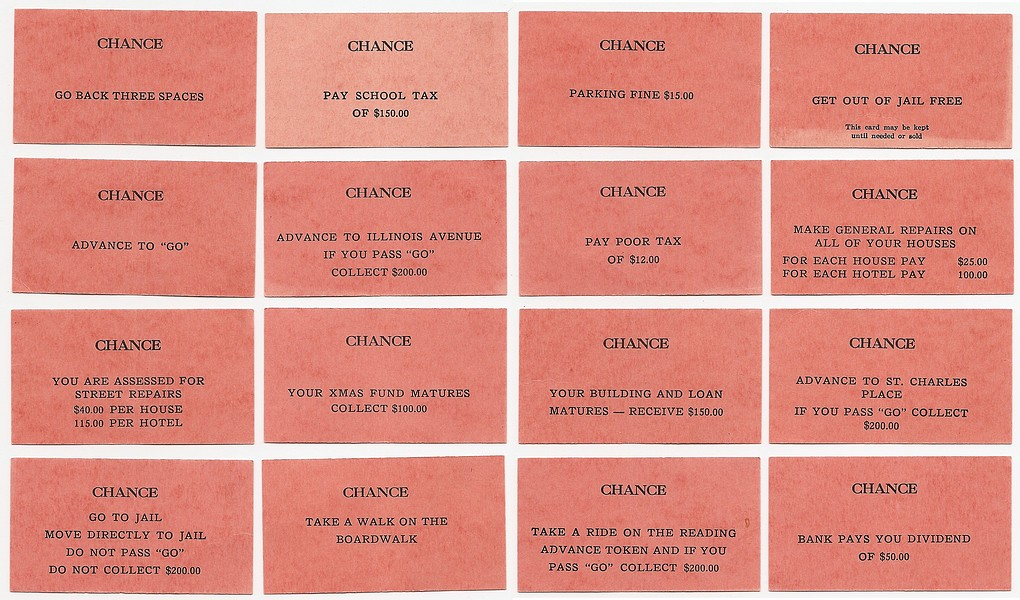
\includegraphics{monopoly_3.jpg}
\caption{chance}
\end{figure}

    Because we are only determining the probabilities, we are only
interested in the following cards:

\begin{itemize}
\tightlist
\item
  go back three spaces
\item
  get out of jail free
\item
  advance to go
\item
  advance to illinois avenue (R3)
\item
  go to jail
\end{itemize}

    \hypertarget{chance-deck-implementation}{%
\subsubsection{Chance deck
implementation}\label{chance-deck-implementation}}

    We implement the chance deck in a class. The class keeps track of a list
with \(16\) cards. An index points to the next card. When we are out of
cards, we reset the index and reshuffle the cards.

    \begin{Verbatim}[commandchars=\\\{\}]
{\color{incolor}In [{\color{incolor}15}]:} \PY{k+kn}{from} \PY{n+nn}{random} \PY{k}{import} \PY{n}{shuffle}
         
         \PY{k}{class} \PY{n+nc}{ChanceDeck}\PY{p}{(}\PY{p}{)}\PY{p}{:}
             \PY{k}{def} \PY{n+nf}{\PYZus{}\PYZus{}init\PYZus{}\PYZus{}}\PY{p}{(}\PY{n+nb+bp}{self}\PY{p}{)}\PY{p}{:}
                 \PY{n+nb+bp}{self}\PY{o}{.}\PY{n}{deck} \PY{o}{=} \PY{p}{[}\PY{l+m+mi}{0}\PY{p}{]} \PY{o}{*} \PY{l+m+mi}{16}
                 \PY{n+nb+bp}{self}\PY{o}{.}\PY{n}{deck}\PY{p}{[}\PY{l+m+mi}{0}\PY{p}{]} \PY{o}{=} \PY{l+s+s1}{\PYZsq{}}\PY{l+s+s1}{gtg}\PY{l+s+s1}{\PYZsq{}} \PY{c+c1}{\PYZsh{} go to go}
                 \PY{n+nb+bp}{self}\PY{o}{.}\PY{n}{deck}\PY{p}{[}\PY{l+m+mi}{1}\PY{p}{]} \PY{o}{=} \PY{l+s+s1}{\PYZsq{}}\PY{l+s+s1}{gtj}\PY{l+s+s1}{\PYZsq{}} \PY{c+c1}{\PYZsh{} go to jail}
                 \PY{n+nb+bp}{self}\PY{o}{.}\PY{n}{deck}\PY{p}{[}\PY{l+m+mi}{2}\PY{p}{]} \PY{o}{=} \PY{l+s+s1}{\PYZsq{}}\PY{l+s+s1}{goj}\PY{l+s+s1}{\PYZsq{}} \PY{c+c1}{\PYZsh{} get out of jail}
                 \PY{n+nb+bp}{self}\PY{o}{.}\PY{n}{deck}\PY{p}{[}\PY{l+m+mi}{3}\PY{p}{]} \PY{o}{=} \PY{l+s+s1}{\PYZsq{}}\PY{l+s+s1}{gb3}\PY{l+s+s1}{\PYZsq{}} \PY{c+c1}{\PYZsh{} go back 3}
                 \PY{n+nb+bp}{self}\PY{o}{.}\PY{n}{deck}\PY{p}{[}\PY{l+m+mi}{4}\PY{p}{]} \PY{o}{=} \PY{l+s+s1}{\PYZsq{}}\PY{l+s+s1}{r3}\PY{l+s+s1}{\PYZsq{}}  \PY{c+c1}{\PYZsh{} go to red 3 (r3)}
                 \PY{n+nb+bp}{self}\PY{o}{.}\PY{n}{index} \PY{o}{=} \PY{l+m+mi}{16}
             
             \PY{k}{def} \PY{n+nf}{draw\PYZus{}card}\PY{p}{(}\PY{n+nb+bp}{self}\PY{p}{)}\PY{p}{:}
                 \PY{k}{if} \PY{n+nb+bp}{self}\PY{o}{.}\PY{n}{index} \PY{o}{\PYZgt{}}\PY{o}{=} \PY{n+nb}{len}\PY{p}{(}\PY{n+nb+bp}{self}\PY{o}{.}\PY{n}{deck}\PY{p}{)}\PY{p}{:}
                     \PY{n+nb+bp}{self}\PY{o}{.}\PY{n}{index} \PY{o}{=} \PY{l+m+mi}{0}
                     \PY{n}{shuffle}\PY{p}{(}\PY{n+nb+bp}{self}\PY{o}{.}\PY{n}{deck}\PY{p}{)}
                 \PY{n}{card} \PY{o}{=} \PY{n+nb+bp}{self}\PY{o}{.}\PY{n}{deck}\PY{p}{[}\PY{n+nb+bp}{self}\PY{o}{.}\PY{n}{index}\PY{p}{]}
                 \PY{n+nb+bp}{self}\PY{o}{.}\PY{n}{index} \PY{o}{+}\PY{o}{=} \PY{l+m+mi}{1}
                 \PY{k}{return} \PY{n}{card}
\end{Verbatim}


    Now we test it:

    \begin{Verbatim}[commandchars=\\\{\}]
{\color{incolor}In [{\color{incolor}16}]:} \PY{n}{deck} \PY{o}{=} \PY{n}{ChanceDeck}\PY{p}{(}\PY{p}{)}
         \PY{n}{deck}\PY{o}{.}\PY{n}{deck}
\end{Verbatim}


\begin{Verbatim}[commandchars=\\\{\}]
{\color{outcolor}Out[{\color{outcolor}16}]:} ['gtg', 'gtj', 'goj', 'gb3', 'r3', 0, 0, 0, 0, 0, 0, 0, 0, 0, 0, 0]
\end{Verbatim}
            
    \begin{Verbatim}[commandchars=\\\{\}]
{\color{incolor}In [{\color{incolor}17}]:} \PY{n}{deck}\PY{o}{.}\PY{n}{draw\PYZus{}card}\PY{p}{(}\PY{p}{)}
\end{Verbatim}


\begin{Verbatim}[commandchars=\\\{\}]
{\color{outcolor}Out[{\color{outcolor}17}]:} 0
\end{Verbatim}
            
    \begin{Verbatim}[commandchars=\\\{\}]
{\color{incolor}In [{\color{incolor}18}]:} \PY{n}{deck}\PY{o}{.}\PY{n}{deck}
\end{Verbatim}


\begin{Verbatim}[commandchars=\\\{\}]
{\color{outcolor}Out[{\color{outcolor}18}]:} [0, 'gtj', 'gtg', 0, 0, 0, 'gb3', 0, 0, 0, 0, 0, 'r3', 0, 0, 'goj']
\end{Verbatim}
            
    \begin{Verbatim}[commandchars=\\\{\}]
{\color{incolor}In [{\color{incolor}19}]:} \PY{n}{deck}\PY{o}{.}\PY{n}{index}
\end{Verbatim}


\begin{Verbatim}[commandchars=\\\{\}]
{\color{outcolor}Out[{\color{outcolor}19}]:} 1
\end{Verbatim}
            
    \hypertarget{dice}{%
\subsection{Dice}\label{dice}}

    We will be implementing the dice as a class. This allows us to
encapsulate how the result are determined. It makes it easier to
implements other scenarios such as throwing with multiple dices.

    \begin{Verbatim}[commandchars=\\\{\}]
{\color{incolor}In [{\color{incolor}20}]:} \PY{k+kn}{from} \PY{n+nn}{random} \PY{k}{import} \PY{n}{randint}
         
         \PY{k}{class} \PY{n+nc}{Dice}\PY{p}{(}\PY{p}{)}\PY{p}{:}
             \PY{k}{def} \PY{n+nf}{\PYZus{}\PYZus{}init\PYZus{}\PYZus{}}\PY{p}{(}\PY{n+nb+bp}{self}\PY{p}{,} \PY{n}{dices} \PY{o}{=} \PY{l+m+mi}{1}\PY{p}{,} \PY{n}{sides} \PY{o}{=} \PY{l+m+mi}{6}\PY{p}{)}\PY{p}{:}
                 \PY{n+nb+bp}{self}\PY{o}{.}\PY{n}{dices} \PY{o}{=} \PY{n}{dices}
                 \PY{n+nb+bp}{self}\PY{o}{.}\PY{n}{sides} \PY{o}{=} \PY{l+m+mi}{6}
             
             \PY{k}{def} \PY{n+nf}{throw}\PY{p}{(}\PY{n+nb+bp}{self}\PY{p}{)}\PY{p}{:}
                 \PY{k}{return} \PY{n+nb}{sum}\PY{p}{(}\PY{p}{[}\PY{n}{randint}\PY{p}{(}\PY{l+m+mi}{1}\PY{p}{,} \PY{n+nb+bp}{self}\PY{o}{.}\PY{n}{sides}\PY{p}{)} \PY{k}{for} \PY{n}{\PYZus{}} \PY{o+ow}{in} \PY{n+nb}{range}\PY{p}{(}\PY{n+nb+bp}{self}\PY{o}{.}\PY{n}{dices}\PY{p}{)}\PY{p}{]}\PY{p}{)}
\end{Verbatim}


    Rolling one time:

    \begin{Verbatim}[commandchars=\\\{\}]
{\color{incolor}In [{\color{incolor}21}]:} \PY{n}{dice} \PY{o}{=} \PY{n}{Dice}\PY{p}{(}\PY{p}{)}
         \PY{n}{dice}\PY{o}{.}\PY{n}{throw}\PY{p}{(}\PY{p}{)}
\end{Verbatim}


\begin{Verbatim}[commandchars=\\\{\}]
{\color{outcolor}Out[{\color{outcolor}21}]:} 1
\end{Verbatim}
            
    \hypertarget{simple-one-dice-with-six-sides}{%
\subsubsection{Simple: one dice with six
sides}\label{simple-one-dice-with-six-sides}}

    A simple setup would be one dice with six sides. This will give
uniformly distributed probabilities.

    \begin{Verbatim}[commandchars=\\\{\}]
{\color{incolor}In [{\color{incolor}88}]:} \PY{n}{dice} \PY{o}{=} \PY{n}{Dice}\PY{p}{(}\PY{p}{)}
         \PY{n}{sides} \PY{o}{=} \PY{p}{[}\PY{l+m+mi}{0}\PY{p}{]} \PY{o}{*} \PY{n}{dice}\PY{o}{.}\PY{n}{dices} \PY{o}{*} \PY{n}{dice}\PY{o}{.}\PY{n}{sides}
         \PY{n}{N} \PY{o}{=} \PY{l+m+mi}{10000}
         \PY{k}{for} \PY{n}{i} \PY{o+ow}{in} \PY{n+nb}{range}\PY{p}{(}\PY{n}{N}\PY{p}{)}\PY{p}{:} \PY{n}{sides}\PY{p}{[}\PY{n}{dice}\PY{o}{.}\PY{n}{throw}\PY{p}{(}\PY{p}{)}\PY{o}{\PYZhy{}}\PY{l+m+mi}{1}\PY{p}{]} \PY{o}{+}\PY{o}{=} \PY{l+m+mi}{1}
         \PY{n}{sides} \PY{o}{=} \PY{n}{np}\PY{o}{.}\PY{n}{array}\PY{p}{(}\PY{n}{sides}\PY{p}{)} \PY{o}{/} \PY{n}{N}
         \PY{n}{bar}\PY{p}{(}\PY{n+nb}{range}\PY{p}{(}\PY{l+m+mi}{1}\PY{p}{,}\PY{n+nb}{len}\PY{p}{(}\PY{n}{sides}\PY{p}{)}\PY{o}{+}\PY{l+m+mi}{1}\PY{p}{)}\PY{p}{,} \PY{n}{sides}\PY{p}{)}\PY{p}{;}
         \PY{n}{ylabel}\PY{p}{(}\PY{l+s+s1}{\PYZsq{}}\PY{l+s+s1}{P(x)}\PY{l+s+s1}{\PYZsq{}}\PY{p}{)}
         \PY{n}{xlabel}\PY{p}{(}\PY{l+s+s1}{\PYZsq{}}\PY{l+s+s1}{x}\PY{l+s+s1}{\PYZsq{}}\PY{p}{)}
         \PY{n}{title}\PY{p}{(}\PY{l+s+s1}{\PYZsq{}}\PY{l+s+s1}{Probability distribution for one dice; N=10,000}\PY{l+s+s1}{\PYZsq{}}\PY{p}{)}\PY{p}{;}
\end{Verbatim}


    \begin{center}
    \adjustimage{max size={0.9\linewidth}{0.9\paperheight}}{output_58_0.png}
    \end{center}
    { \hspace*{\fill} \\}
    
    \hypertarget{advanced-two-dice-with-six-sides}{%
\subsubsection{Advanced: two dice with six
sides}\label{advanced-two-dice-with-six-sides}}

    Monopoly is played with two dices. This will the following probability
distribution:

    \begin{Verbatim}[commandchars=\\\{\}]
{\color{incolor}In [{\color{incolor}89}]:} \PY{n}{dice} \PY{o}{=} \PY{n}{Dice}\PY{p}{(}\PY{l+m+mi}{2}\PY{p}{)}
         \PY{n}{sides} \PY{o}{=} \PY{p}{[}\PY{l+m+mi}{0}\PY{p}{]} \PY{o}{*} \PY{n}{dice}\PY{o}{.}\PY{n}{dices} \PY{o}{*} \PY{n}{dice}\PY{o}{.}\PY{n}{sides}
         \PY{n}{N} \PY{o}{=} \PY{l+m+mi}{10000}
         \PY{k}{for} \PY{n}{i} \PY{o+ow}{in} \PY{n+nb}{range}\PY{p}{(}\PY{n}{N}\PY{p}{)}\PY{p}{:} \PY{n}{sides}\PY{p}{[}\PY{n}{dice}\PY{o}{.}\PY{n}{throw}\PY{p}{(}\PY{p}{)}\PY{o}{\PYZhy{}}\PY{l+m+mi}{1}\PY{p}{]} \PY{o}{+}\PY{o}{=} \PY{l+m+mi}{1}
         \PY{n}{sides} \PY{o}{=} \PY{n}{np}\PY{o}{.}\PY{n}{array}\PY{p}{(}\PY{n}{sides}\PY{p}{)} \PY{o}{/} \PY{n}{N}
         \PY{n}{bar}\PY{p}{(}\PY{n+nb}{range}\PY{p}{(}\PY{l+m+mi}{1}\PY{p}{,}\PY{n+nb}{len}\PY{p}{(}\PY{n}{sides}\PY{p}{)}\PY{o}{+}\PY{l+m+mi}{1}\PY{p}{)}\PY{p}{,} \PY{n}{sides}\PY{p}{)}\PY{p}{;}
         \PY{n}{ylabel}\PY{p}{(}\PY{l+s+s1}{\PYZsq{}}\PY{l+s+s1}{P(x)}\PY{l+s+s1}{\PYZsq{}}\PY{p}{)}
         \PY{n}{xlabel}\PY{p}{(}\PY{l+s+s1}{\PYZsq{}}\PY{l+s+s1}{x}\PY{l+s+s1}{\PYZsq{}}\PY{p}{)}
         \PY{n}{title}\PY{p}{(}\PY{l+s+s1}{\PYZsq{}}\PY{l+s+s1}{Probability distribution for two dices; N=10,000}\PY{l+s+s1}{\PYZsq{}}\PY{p}{)}\PY{p}{;}
\end{Verbatim}


    \begin{center}
    \adjustimage{max size={0.9\linewidth}{0.9\paperheight}}{output_61_0.png}
    \end{center}
    { \hspace*{\fill} \\}
    
    \hypertarget{monopoly-simulation}{%
\subsection{Monopoly simulation}\label{monopoly-simulation}}

    We are playing a simplified version of Monopoly. We will not keep track
of money. There will only be one player. If a player goes to jail, the
player can continue immediately on the next turn. We will keep track of
the card decks. The game will be played with \(2\) dices. We only count
when we land on a square. If we are moved to jail for example, the next
round will continue from that new position.

    \hypertarget{algorithm}{%
\subsubsection{Algorithm}\label{algorithm}}

    Here we are going to simulate a game for \(N\) amount of rounds. The
game algorithm is simple:

\begin{enumerate}
\def\labelenumi{\arabic{enumi}.}
\tightlist
\item
  Roll the dices (there are \(2\) dices with \(6\) squares)
\item
  Move to the new position
\item
  Increment the square counter for that position
\item
  Check and handle go to jail
\item
  Check and handle community chest
\item
  Check and handle chance
\end{enumerate}

    \hypertarget{modulo-arithmetic-for-position-tracking}{%
\subsubsection{Modulo arithmetic for position
tracking}\label{modulo-arithmetic-for-position-tracking}}

    We can easily keep track of our position with modulo arithemetic. Let
\(C\) be our position (or \texttt{index}), \(d\) the result from
throwing the dice, and \(n\) the current round. To determine our new
position we calculate:

\[ C_{n+1} \equiv C_n+d \pmod{40}\]

    The modulo is \(40\) because that are the total amount of squares.

    \hypertarget{implementation}{%
\subsubsection{Implementation}\label{implementation}}

    Below is the implementation for the Monopoly simulation.

    \begin{Verbatim}[commandchars=\\\{\}]
{\color{incolor}In [{\color{incolor}90}]:} \PY{n}{dice} \PY{o}{=} \PY{n}{Dice}\PY{p}{(}\PY{l+m+mi}{2}\PY{p}{)}
         \PY{n}{community\PYZus{}deck} \PY{o}{=} \PY{n}{CommunityDeck}\PY{p}{(}\PY{p}{)}
         \PY{n}{chance\PYZus{}deck} \PY{o}{=} \PY{n}{ChanceDeck}\PY{p}{(}\PY{p}{)}
         
         \PY{n}{index} \PY{o}{=} \PY{l+m+mi}{0} \PY{c+c1}{\PYZsh{} position}
         \PY{n}{total\PYZus{}squares} \PY{o}{=} \PY{n+nb}{len}\PY{p}{(}\PY{n}{squares\PYZus{}labels}\PY{p}{)}
         \PY{n}{squares} \PY{o}{=} \PY{p}{[}\PY{l+m+mi}{0}\PY{p}{]} \PY{o}{*} \PY{n}{total\PYZus{}squares}
         
         \PY{n}{rounds} \PY{o}{=} \PY{l+m+mi}{1000000} \PY{c+c1}{\PYZsh{} N}
         
         \PY{k}{for} \PY{n}{i} \PY{o+ow}{in} \PY{n+nb}{range}\PY{p}{(}\PY{n}{rounds}\PY{p}{)}\PY{p}{:}
             
             \PY{c+c1}{\PYZsh{} Throw the dice and move our position on the board.}
             \PY{n}{steps} \PY{o}{=} \PY{n}{dice}\PY{o}{.}\PY{n}{throw}\PY{p}{(}\PY{p}{)}
             \PY{n}{index} \PY{o}{=} \PY{p}{(}\PY{n}{index} \PY{o}{+} \PY{n}{steps}\PY{p}{)} \PY{o}{\PYZpc{}} \PY{n}{total\PYZus{}squares}
             \PY{n}{squares}\PY{p}{[}\PY{n}{index}\PY{p}{]} \PY{o}{+}\PY{o}{=} \PY{l+m+mi}{1}
             
             \PY{c+c1}{\PYZsh{} We landed on go to jail.}
             \PY{k}{if} \PY{n}{squares\PYZus{}labels}\PY{p}{[}\PY{n}{index}\PY{p}{]} \PY{o+ow}{is} \PY{l+s+s1}{\PYZsq{}}\PY{l+s+s1}{gtj}\PY{l+s+s1}{\PYZsq{}}\PY{p}{:} 
                 \PY{n}{index} \PY{o}{=} \PY{n}{squares\PYZus{}labels}\PY{o}{.}\PY{n}{index}\PY{p}{(}\PY{l+s+s1}{\PYZsq{}}\PY{l+s+s1}{jail}\PY{l+s+s1}{\PYZsq{}}\PY{p}{)}
             
             \PY{c+c1}{\PYZsh{} We landed on the community card.}
             \PY{k}{if} \PY{n}{squares\PYZus{}labels}\PY{p}{[}\PY{n}{index}\PY{p}{]} \PY{o+ow}{in} \PY{p}{[}\PY{l+s+s1}{\PYZsq{}}\PY{l+s+s1}{cc1}\PY{l+s+s1}{\PYZsq{}}\PY{p}{,} \PY{l+s+s1}{\PYZsq{}}\PY{l+s+s1}{cc2}\PY{l+s+s1}{\PYZsq{}}\PY{p}{,} \PY{l+s+s1}{\PYZsq{}}\PY{l+s+s1}{cc3}\PY{l+s+s1}{\PYZsq{}}\PY{p}{]}\PY{p}{:}
                 \PY{n}{card} \PY{o}{=} \PY{n}{community\PYZus{}deck}\PY{o}{.}\PY{n}{draw\PYZus{}card}\PY{p}{(}\PY{p}{)}
                 \PY{k}{if} \PY{n}{card} \PY{o+ow}{is} \PY{l+s+s1}{\PYZsq{}}\PY{l+s+s1}{gtg}\PY{l+s+s1}{\PYZsq{}}\PY{p}{:} \PY{n}{index} \PY{o}{=} \PY{n}{squares\PYZus{}labels}\PY{o}{.}\PY{n}{index}\PY{p}{(}\PY{l+s+s1}{\PYZsq{}}\PY{l+s+s1}{start}\PY{l+s+s1}{\PYZsq{}}\PY{p}{)}
                 \PY{k}{if} \PY{n}{card} \PY{o+ow}{is} \PY{l+s+s1}{\PYZsq{}}\PY{l+s+s1}{gtj}\PY{l+s+s1}{\PYZsq{}}\PY{p}{:} \PY{n}{index} \PY{o}{=} \PY{n}{squares\PYZus{}labels}\PY{o}{.}\PY{n}{index}\PY{p}{(}\PY{l+s+s1}{\PYZsq{}}\PY{l+s+s1}{jail}\PY{l+s+s1}{\PYZsq{}}\PY{p}{)}
                 \PY{k}{if} \PY{n}{card} \PY{o+ow}{is} \PY{l+s+s1}{\PYZsq{}}\PY{l+s+s1}{gb2}\PY{l+s+s1}{\PYZsq{}}\PY{p}{:} 
                     \PY{k}{if} \PY{n}{index} \PY{o}{\PYZgt{}}\PY{o}{=} \PY{l+m+mi}{2}\PY{p}{:} \PY{n}{index} \PY{o}{\PYZhy{}}\PY{o}{=} \PY{l+m+mi}{2}
                     \PY{k}{if} \PY{n}{index} \PY{o}{\PYZlt{}} \PY{l+m+mi}{2}\PY{p}{:} \PY{n}{index} \PY{o}{=} \PY{n}{total\PYZus{}squares}\PY{o}{\PYZhy{}}\PY{n+nb}{abs}\PY{p}{(}\PY{n}{index}\PY{o}{\PYZhy{}}\PY{l+m+mi}{2}\PY{p}{)}\PY{o}{\PYZhy{}}\PY{l+m+mi}{1}
             
             \PY{c+c1}{\PYZsh{} We landed on the chance card.}
             \PY{k}{if} \PY{n}{squares\PYZus{}labels}\PY{p}{[}\PY{n}{index}\PY{p}{]} \PY{o+ow}{in} \PY{p}{[}\PY{l+s+s1}{\PYZsq{}}\PY{l+s+s1}{c1}\PY{l+s+s1}{\PYZsq{}}\PY{p}{,} \PY{l+s+s1}{\PYZsq{}}\PY{l+s+s1}{c2}\PY{l+s+s1}{\PYZsq{}}\PY{p}{,} \PY{l+s+s1}{\PYZsq{}}\PY{l+s+s1}{c3}\PY{l+s+s1}{\PYZsq{}}\PY{p}{]}\PY{p}{:}
                 \PY{n}{card} \PY{o}{=} \PY{n}{chance\PYZus{}deck}\PY{o}{.}\PY{n}{draw\PYZus{}card}\PY{p}{(}\PY{p}{)}
                 \PY{k}{if} \PY{n}{card} \PY{o+ow}{is} \PY{l+s+s1}{\PYZsq{}}\PY{l+s+s1}{gtg}\PY{l+s+s1}{\PYZsq{}}\PY{p}{:} \PY{n}{index} \PY{o}{=} \PY{n}{squares\PYZus{}labels}\PY{o}{.}\PY{n}{index}\PY{p}{(}\PY{l+s+s1}{\PYZsq{}}\PY{l+s+s1}{start}\PY{l+s+s1}{\PYZsq{}}\PY{p}{)}
                 \PY{k}{if} \PY{n}{card} \PY{o+ow}{is} \PY{l+s+s1}{\PYZsq{}}\PY{l+s+s1}{gtj}\PY{l+s+s1}{\PYZsq{}}\PY{p}{:} \PY{n}{index} \PY{o}{=} \PY{n}{squares\PYZus{}labels}\PY{o}{.}\PY{n}{index}\PY{p}{(}\PY{l+s+s1}{\PYZsq{}}\PY{l+s+s1}{jail}\PY{l+s+s1}{\PYZsq{}}\PY{p}{)}
                 \PY{k}{if} \PY{n}{card} \PY{o+ow}{is} \PY{l+s+s1}{\PYZsq{}}\PY{l+s+s1}{r3}\PY{l+s+s1}{\PYZsq{}}\PY{p}{:} \PY{n}{index} \PY{o}{=} \PY{n}{squares\PYZus{}labels}\PY{o}{.}\PY{n}{index}\PY{p}{(}\PY{l+s+s1}{\PYZsq{}}\PY{l+s+s1}{r3}\PY{l+s+s1}{\PYZsq{}}\PY{p}{)}
                 \PY{k}{if} \PY{n}{card} \PY{o+ow}{is} \PY{l+s+s1}{\PYZsq{}}\PY{l+s+s1}{gb3}\PY{l+s+s1}{\PYZsq{}}\PY{p}{:}
                     \PY{k}{if} \PY{n}{index} \PY{o}{\PYZgt{}}\PY{o}{=} \PY{l+m+mi}{3}\PY{p}{:} \PY{n}{index} \PY{o}{\PYZhy{}}\PY{o}{=} \PY{l+m+mi}{3}
                     \PY{k}{if} \PY{n}{index} \PY{o}{\PYZlt{}} \PY{l+m+mi}{3}\PY{p}{:} \PY{n}{index} \PY{o}{=} \PY{n}{total\PYZus{}squares}\PY{o}{\PYZhy{}}\PY{n+nb}{abs}\PY{p}{(}\PY{n}{index}\PY{o}{\PYZhy{}}\PY{l+m+mi}{3}\PY{p}{)}\PY{o}{\PYZhy{}}\PY{l+m+mi}{1}
\end{Verbatim}


    It takes around \(2.7\) seconds to run a game when \(N=1,000,000\).
Because there is only one loop the algorithm will scale linearly.

    \hypertarget{probability-statistics}{%
\subsection{Probability statistics}\label{probability-statistics}}

    Now we can proceed to analyze our results.

    \hypertarget{determining-probabilities}{%
\subsubsection{Determining
probabilities}\label{determining-probabilities}}

    With the number of times that each square is visited we can calculate
the probabilities. The probability that a square is visited is:

\[ P(\bar{x}=x) = \dfrac{\text{Times visited}}{\text{\# of rounds}} \]

    We can calculate the expected value for each square in terms of money
with:

    \[ E(\bar{k}) = P(\bar{x}=x)\cdot\text{Rent} \]

    We also want to create a \texttt{DataFrame} in Python to easily keep
track of everything.

    \begin{Verbatim}[commandchars=\\\{\}]
{\color{incolor}In [{\color{incolor}25}]:} \PY{k+kn}{import} \PY{n+nn}{pandas} \PY{k}{as} \PY{n+nn}{pd}
         \PY{n}{df} \PY{o}{=} \PY{n}{pd}\PY{o}{.}\PY{n}{DataFrame}\PY{p}{(}\PY{n}{index}\PY{o}{=}\PY{n+nb}{range}\PY{p}{(}\PY{n}{total\PYZus{}squares}\PY{p}{)}\PY{p}{)}
         \PY{n}{df}\PY{p}{[}\PY{l+s+s1}{\PYZsq{}}\PY{l+s+s1}{Square}\PY{l+s+s1}{\PYZsq{}}\PY{p}{]} \PY{o}{=} \PY{n}{squares\PYZus{}labels}
         \PY{n}{df}\PY{p}{[}\PY{l+s+s1}{\PYZsq{}}\PY{l+s+s1}{Description}\PY{l+s+s1}{\PYZsq{}}\PY{p}{]} \PY{o}{=} \PY{n}{squares\PYZus{}description}
         \PY{n}{df}\PY{p}{[}\PY{l+s+s1}{\PYZsq{}}\PY{l+s+s1}{Purchasable}\PY{l+s+s1}{\PYZsq{}}\PY{p}{]} \PY{o}{=} \PY{n}{squares\PYZus{}purchasable}
         \PY{n}{df}\PY{p}{[}\PY{l+s+s1}{\PYZsq{}}\PY{l+s+s1}{Rent}\PY{l+s+s1}{\PYZsq{}}\PY{p}{]} \PY{o}{=} \PY{n}{squares\PYZus{}rent}
         \PY{n}{df}\PY{p}{[}\PY{l+s+s1}{\PYZsq{}}\PY{l+s+s1}{Visited}\PY{l+s+s1}{\PYZsq{}}\PY{p}{]} \PY{o}{=} \PY{n}{squares}
         \PY{n}{df}\PY{p}{[}\PY{l+s+s1}{\PYZsq{}}\PY{l+s+s1}{Probability}\PY{l+s+s1}{\PYZsq{}}\PY{p}{]} \PY{o}{=} \PY{n}{df}\PY{p}{[}\PY{l+s+s1}{\PYZsq{}}\PY{l+s+s1}{Visited}\PY{l+s+s1}{\PYZsq{}}\PY{p}{]} \PY{o}{/} \PY{n}{rounds}
         \PY{n}{df}\PY{p}{[}\PY{l+s+s1}{\PYZsq{}}\PY{l+s+s1}{Aggregate}\PY{l+s+s1}{\PYZsq{}}\PY{p}{]} \PY{o}{=} \PY{n}{squares\PYZus{}aggregate}
         \PY{n}{df}\PY{p}{[}\PY{l+s+s1}{\PYZsq{}}\PY{l+s+s1}{Expected Value}\PY{l+s+s1}{\PYZsq{}}\PY{p}{]} \PY{o}{=} \PY{n}{df}\PY{p}{[}\PY{l+s+s1}{\PYZsq{}}\PY{l+s+s1}{Probability}\PY{l+s+s1}{\PYZsq{}}\PY{p}{]} \PY{o}{*} \PY{n}{df}\PY{p}{[}\PY{l+s+s1}{\PYZsq{}}\PY{l+s+s1}{Rent}\PY{l+s+s1}{\PYZsq{}}\PY{p}{]}
\end{Verbatim}


    We can calculate a quick summary about the data:

    \begin{Verbatim}[commandchars=\\\{\}]
{\color{incolor}In [{\color{incolor}26}]:} \PY{n+nb}{print}\PY{p}{(}\PY{l+s+s1}{\PYZsq{}}\PY{l+s+s1}{Total rounds: }\PY{l+s+si}{\PYZob{}\PYZcb{}}\PY{l+s+s1}{\PYZsq{}}\PY{o}{.}\PY{n}{format}\PY{p}{(}\PY{n}{rounds}\PY{p}{)}\PY{p}{)}
         \PY{n+nb}{print}\PY{p}{(}\PY{l+s+s1}{\PYZsq{}}\PY{l+s+s1}{Visited avg:  }\PY{l+s+si}{\PYZob{}\PYZcb{}}\PY{l+s+s1}{\PYZsq{}}\PY{o}{.}\PY{n}{format}\PY{p}{(}\PY{n}{df}\PY{p}{[}\PY{l+s+s1}{\PYZsq{}}\PY{l+s+s1}{Visited}\PY{l+s+s1}{\PYZsq{}}\PY{p}{]}\PY{o}{.}\PY{n}{mean}\PY{p}{(}\PY{p}{)}\PY{p}{)}\PY{p}{)}
         \PY{n+nb}{print}\PY{p}{(}\PY{l+s+s1}{\PYZsq{}}\PY{l+s+s1}{Visited min:  }\PY{l+s+si}{\PYZob{}\PYZcb{}}\PY{l+s+s1}{\PYZsq{}}\PY{o}{.}\PY{n}{format}\PY{p}{(}\PY{n}{df}\PY{p}{[}\PY{l+s+s1}{\PYZsq{}}\PY{l+s+s1}{Visited}\PY{l+s+s1}{\PYZsq{}}\PY{p}{]}\PY{o}{.}\PY{n}{min}\PY{p}{(}\PY{p}{)}\PY{p}{)}\PY{p}{)}
         \PY{n+nb}{print}\PY{p}{(}\PY{l+s+s1}{\PYZsq{}}\PY{l+s+s1}{Visited max:  }\PY{l+s+si}{\PYZob{}\PYZcb{}}\PY{l+s+s1}{\PYZsq{}}\PY{o}{.}\PY{n}{format}\PY{p}{(}\PY{n}{df}\PY{p}{[}\PY{l+s+s1}{\PYZsq{}}\PY{l+s+s1}{Visited}\PY{l+s+s1}{\PYZsq{}}\PY{p}{]}\PY{o}{.}\PY{n}{max}\PY{p}{(}\PY{p}{)}\PY{p}{)}\PY{p}{)}
         \PY{n+nb}{print}\PY{p}{(}\PY{l+s+s1}{\PYZsq{}}\PY{l+s+s1}{Visited std:  }\PY{l+s+si}{\PYZob{}:.2f\PYZcb{}}\PY{l+s+s1}{\PYZsq{}}\PY{o}{.}\PY{n}{format}\PY{p}{(}\PY{n}{df}\PY{p}{[}\PY{l+s+s1}{\PYZsq{}}\PY{l+s+s1}{Visited}\PY{l+s+s1}{\PYZsq{}}\PY{p}{]}\PY{o}{.}\PY{n}{std}\PY{p}{(}\PY{p}{)}\PY{p}{)}\PY{p}{)}
\end{Verbatim}


    \begin{Verbatim}[commandchars=\\\{\}]
Total rounds: 1000000
Visited avg:  25000.0
Visited min:  21973
Visited max:  28895
Visited std:  2175.56

    \end{Verbatim}

    \hypertarget{plot-of-probabilities-by-square}{%
\subsubsection{Plot of probabilities by
square}\label{plot-of-probabilities-by-square}}

    If we sort these values descending on the probability, we can easily see
which squares have the highest probability to be visited.

    \begin{Verbatim}[commandchars=\\\{\}]
{\color{incolor}In [{\color{incolor}27}]:} \PY{n}{plt}\PY{o}{.}\PY{n}{rc}\PY{p}{(}\PY{l+s+s1}{\PYZsq{}}\PY{l+s+s1}{xtick}\PY{l+s+s1}{\PYZsq{}}\PY{p}{,} \PY{n}{labelsize}\PY{o}{=}\PY{l+m+mi}{16}\PY{p}{)} 
         \PY{n}{plt}\PY{o}{.}\PY{n}{rc}\PY{p}{(}\PY{l+s+s1}{\PYZsq{}}\PY{l+s+s1}{ytick}\PY{l+s+s1}{\PYZsq{}}\PY{p}{,} \PY{n}{labelsize}\PY{o}{=}\PY{l+m+mi}{14}\PY{p}{)} 
         \PY{n}{df}\PY{p}{[}\PY{p}{[}\PY{l+s+s1}{\PYZsq{}}\PY{l+s+s1}{Description}\PY{l+s+s1}{\PYZsq{}}\PY{p}{,} \PY{l+s+s1}{\PYZsq{}}\PY{l+s+s1}{Probability}\PY{l+s+s1}{\PYZsq{}}\PY{p}{]}\PY{p}{]}\PY{o}{.}\PY{n}{sort\PYZus{}values}\PY{p}{(}\PY{n}{by}\PY{o}{=}\PY{l+s+s1}{\PYZsq{}}\PY{l+s+s1}{Probability}\PY{l+s+s1}{\PYZsq{}}\PY{p}{,} \PY{n}{ascending}\PY{o}{=}\PY{k+kc}{False}\PY{p}{)}\PYZbs{}
             \PY{o}{.}\PY{n}{plot}\PY{p}{(}\PY{n}{kind}\PY{o}{=}\PY{l+s+s1}{\PYZsq{}}\PY{l+s+s1}{bar}\PY{l+s+s1}{\PYZsq{}}\PY{p}{,} \PY{n}{figsize}\PY{o}{=}\PY{p}{(}\PY{l+m+mi}{20}\PY{p}{,}\PY{l+m+mi}{5}\PY{p}{)}\PY{p}{)}
         \PY{n}{plt}\PY{o}{.}\PY{n}{xticks}\PY{p}{(}\PY{n+nb}{range}\PY{p}{(}\PY{n}{total\PYZus{}squares}\PY{p}{)}\PY{p}{,} \PY{n}{df}\PY{p}{[}\PY{p}{[}\PY{l+s+s1}{\PYZsq{}}\PY{l+s+s1}{Description}\PY{l+s+s1}{\PYZsq{}}\PY{p}{,} \PY{l+s+s1}{\PYZsq{}}\PY{l+s+s1}{Probability}\PY{l+s+s1}{\PYZsq{}}\PY{p}{]}\PY{p}{]}
             \PY{o}{.}\PY{n}{sort\PYZus{}values}\PY{p}{(}\PY{n}{by}\PY{o}{=}\PY{l+s+s1}{\PYZsq{}}\PY{l+s+s1}{Probability}\PY{l+s+s1}{\PYZsq{}}\PY{p}{,} \PY{n}{ascending}\PY{o}{=}\PY{k+kc}{False}\PY{p}{)}\PY{p}{[}\PY{l+s+s1}{\PYZsq{}}\PY{l+s+s1}{Description}\PY{l+s+s1}{\PYZsq{}}\PY{p}{]}\PY{p}{)}
         \PY{n}{plt}\PY{o}{.}\PY{n}{ylabel}\PY{p}{(}\PY{l+s+s1}{\PYZsq{}}\PY{l+s+s1}{Probability}\PY{l+s+s1}{\PYZsq{}}\PY{p}{)}
         \PY{n}{plt}\PY{o}{.}\PY{n}{title}\PY{p}{(}\PY{l+s+s1}{\PYZsq{}}\PY{l+s+s1}{Probability by Square}\PY{l+s+s1}{\PYZsq{}}\PY{p}{)}\PY{p}{;}
\end{Verbatim}


    \begin{center}
    \adjustimage{max size={0.9\linewidth}{0.9\paperheight}}{output_85_0.png}
    \end{center}
    { \hspace*{\fill} \\}
    
    Here we can conclude that \texttt{Orange\ 1} is the most visited square.
Also notice that \texttt{Orange\ 2} and \texttt{Orange\ 3} are pretty
high. It seems that \texttt{Orange} is the best street to have.

\hypertarget{table-of-probabilities-by-square}{%
\subsubsection{Table of probabilities by
square}\label{table-of-probabilities-by-square}}

Below is the full table with all the squares and their corresponding
values.

    \begin{Verbatim}[commandchars=\\\{\}]
{\color{incolor}In [{\color{incolor}102}]:} \PY{n}{df}\PY{o}{.}\PY{n}{loc}\PY{p}{[}\PY{p}{:}\PY{p}{,} \PY{n}{df}\PY{o}{.}\PY{n}{columns}\PY{o}{.}\PY{n}{isin}\PY{p}{(}\PY{p}{[}\PY{l+s+s1}{\PYZsq{}}\PY{l+s+s1}{Square}\PY{l+s+s1}{\PYZsq{}}\PY{p}{,} \PY{l+s+s1}{\PYZsq{}}\PY{l+s+s1}{Description}\PY{l+s+s1}{\PYZsq{}}\PY{p}{,} \PY{l+s+s1}{\PYZsq{}}\PY{l+s+s1}{Probability}\PY{l+s+s1}{\PYZsq{}}\PY{p}{]}\PY{p}{)}\PY{p}{]}\PY{o}{.}\PY{n}{sort\PYZus{}values}\PY{p}{(}\PY{n}{by}\PY{o}{=}\PY{l+s+s1}{\PYZsq{}}\PY{l+s+s1}{Probability}\PY{l+s+s1}{\PYZsq{}}\PY{p}{,} \PY{n}{ascending}\PY{o}{=}\PY{k+kc}{False}\PY{p}{)}
\end{Verbatim}


\begin{Verbatim}[commandchars=\\\{\}]
{\color{outcolor}Out[{\color{outcolor}102}]:}    Square        Description  Probability
          17    cc2  Community Chest 2     0.028895
          18     o2           Orange 2     0.028447
          19     o3           Orange 3     0.028035
          16     o1           Orange 1     0.027736
          20      p       Free Parking     0.027539
          21     r1              Red 1     0.027316
          26     y1           Yellow 1     0.027288
          22     c2           Chance 2     0.026892
          23     r2              Red 2     0.026878
          27     y2           Yellow 2     0.026876
          30    gtj         Go to Jail     0.026837
          31     g1            Green 1     0.026799
          28     ww        Water Works     0.026769
          29     y3           Yellow 3     0.026719
          25    ts3    Train Station 3     0.026718
          24     r3              Red 3     0.026641
          15    ts2    Train Station 2     0.026571
          32     g2            Green 2     0.026236
          33    cc3  Community Chest 3     0.025676
          14     p3           Purple 3     0.025082
          34     g3            Green 3     0.024969
          13     p2           Purple 2     0.024221
          35    ts4    Train Station 4     0.023904
          7      c1           Chance 1     0.023619
          12     ec   Electric Company     0.023254
          8     lb2       Light Blue 2     0.023096
          10   jail               Jail     0.023040
          36     c3           Chance 3     0.023013
          5      t1    Train Station 1     0.023001
          4      it         Income Tax     0.022989
          6     lb1       Light Blue 1     0.022955
          3      b2            Brown 2     0.022941
          9     lb3       Light Blue 3     0.022853
          11     p1           Purple 1     0.022802
          2     cc1  Community Chest 1     0.022639
          1      b1            Brown 1     0.022416
          38     st          Super Tax     0.022214
          0   start              Start     0.022133
          37    db1        Dark Blue 1     0.022018
          39    db2        Dark Blue 2     0.021973
\end{Verbatim}
            
    \hypertarget{top-10-highest-probability-squares}{%
\subsubsection{Top 10 highest probability
squares}\label{top-10-highest-probability-squares}}

    The top 10 squares that have the highest probability for a player to
land on are:

    \begin{Verbatim}[commandchars=\\\{\}]
{\color{incolor}In [{\color{incolor}101}]:} \PY{n}{df}\PY{o}{.}\PY{n}{loc}\PY{p}{[}\PY{n}{df}\PY{p}{[}\PY{l+s+s1}{\PYZsq{}}\PY{l+s+s1}{Purchasable}\PY{l+s+s1}{\PYZsq{}}\PY{p}{]} \PY{o}{==} \PY{k+kc}{True}\PY{p}{,} \PY{n}{df}\PY{o}{.}\PY{n}{columns}\PY{o}{.}\PY{n}{isin}\PY{p}{(}\PY{p}{[}\PY{l+s+s1}{\PYZsq{}}\PY{l+s+s1}{Square}\PY{l+s+s1}{\PYZsq{}}\PY{p}{,} \PY{l+s+s1}{\PYZsq{}}\PY{l+s+s1}{Description}\PY{l+s+s1}{\PYZsq{}}\PY{p}{,} \PY{l+s+s1}{\PYZsq{}}\PY{l+s+s1}{Probability}\PY{l+s+s1}{\PYZsq{}}\PY{p}{]}\PY{p}{)}\PY{p}{]}\PYZbs{}
              \PY{o}{.}\PY{n}{sort\PYZus{}values}\PY{p}{(}\PY{l+s+s1}{\PYZsq{}}\PY{l+s+s1}{Probability}\PY{l+s+s1}{\PYZsq{}}\PY{p}{,} \PY{n}{ascending}\PY{o}{=}\PY{k+kc}{False}\PY{p}{)}\PY{o}{.}\PY{n}{head}\PY{p}{(}\PY{l+m+mi}{10}\PY{p}{)}
\end{Verbatim}


\begin{Verbatim}[commandchars=\\\{\}]
{\color{outcolor}Out[{\color{outcolor}101}]:}    Square  Description  Probability
          18     o2     Orange 2     0.028447
          19     o3     Orange 3     0.028035
          16     o1     Orange 1     0.027736
          21     r1        Red 1     0.027316
          26     y1     Yellow 1     0.027288
          23     r2        Red 2     0.026878
          27     y2     Yellow 2     0.026876
          31     g1      Green 1     0.026799
          28     ww  Water Works     0.026769
          29     y3     Yellow 3     0.026719
\end{Verbatim}
            
    The total probability for all 10 squares is:

    \begin{Verbatim}[commandchars=\\\{\}]
{\color{incolor}In [{\color{incolor}30}]:} \PY{n}{df}\PY{o}{.}\PY{n}{loc}\PY{p}{[}\PY{n}{df}\PY{p}{[}\PY{l+s+s1}{\PYZsq{}}\PY{l+s+s1}{Purchasable}\PY{l+s+s1}{\PYZsq{}}\PY{p}{]} \PY{o}{==} \PY{k+kc}{True}\PY{p}{]}\PY{o}{.}\PY{n}{sort\PYZus{}values}\PY{p}{(}\PY{l+s+s1}{\PYZsq{}}\PY{l+s+s1}{Probability}\PY{l+s+s1}{\PYZsq{}}\PY{p}{,} \PY{n}{ascending}\PY{o}{=}\PY{k+kc}{False}\PY{p}{)}\PYZbs{}
             \PY{o}{.}\PY{n}{head}\PY{p}{(}\PY{l+m+mi}{10}\PY{p}{)}\PY{p}{[}\PY{l+s+s1}{\PYZsq{}}\PY{l+s+s1}{Probability}\PY{l+s+s1}{\PYZsq{}}\PY{p}{]}\PY{o}{.}\PY{n}{sum}\PY{p}{(}\PY{p}{)}
\end{Verbatim}


\begin{Verbatim}[commandchars=\\\{\}]
{\color{outcolor}Out[{\color{outcolor}30}]:} 0.27286299999999997
\end{Verbatim}
            
    \hypertarget{plot-of-expected-value-per-turn}{%
\subsubsection{Plot of expected value per
turn}\label{plot-of-expected-value-per-turn}}

    Now we want to know how much each square generates per turn with the
found probabilities and the rent the player needs to pay when we land on
it. First we make a selection to only get the purchasable squares.

    \begin{Verbatim}[commandchars=\\\{\}]
{\color{incolor}In [{\color{incolor}31}]:} \PY{n}{rentable\PYZus{}df} \PY{o}{=} \PY{n}{pd}\PY{o}{.}\PY{n}{DataFrame}\PY{p}{(}\PY{n}{df}\PY{o}{.}\PY{n}{loc}\PY{p}{[}\PY{n}{df}\PY{p}{[}\PY{l+s+s1}{\PYZsq{}}\PY{l+s+s1}{Purchasable}\PY{l+s+s1}{\PYZsq{}}\PY{p}{]} \PY{o}{==} \PY{k+kc}{True}\PY{p}{]}\PY{p}{)}\PY{o}{.}\PY{n}{reindex}\PY{p}{(}\PY{p}{)}
\end{Verbatim}


    Plotting this gives:

    \begin{Verbatim}[commandchars=\\\{\}]
{\color{incolor}In [{\color{incolor}32}]:} \PY{n}{plt}\PY{o}{.}\PY{n}{rc}\PY{p}{(}\PY{l+s+s1}{\PYZsq{}}\PY{l+s+s1}{xtick}\PY{l+s+s1}{\PYZsq{}}\PY{p}{,} \PY{n}{labelsize}\PY{o}{=}\PY{l+m+mi}{16}\PY{p}{)} 
         \PY{n}{plt}\PY{o}{.}\PY{n}{rc}\PY{p}{(}\PY{l+s+s1}{\PYZsq{}}\PY{l+s+s1}{ytick}\PY{l+s+s1}{\PYZsq{}}\PY{p}{,} \PY{n}{labelsize}\PY{o}{=}\PY{l+m+mi}{14}\PY{p}{)} 
         \PY{n}{rentable\PYZus{}df}\PY{p}{[}\PY{p}{[}\PY{l+s+s1}{\PYZsq{}}\PY{l+s+s1}{Description}\PY{l+s+s1}{\PYZsq{}}\PY{p}{,} \PY{l+s+s1}{\PYZsq{}}\PY{l+s+s1}{Expected Value}\PY{l+s+s1}{\PYZsq{}}\PY{p}{]}\PY{p}{]}\PY{o}{.}\PY{n}{sort\PYZus{}values}\PY{p}{(}\PY{n}{by}\PY{o}{=}\PY{l+s+s1}{\PYZsq{}}\PY{l+s+s1}{Expected Value}\PY{l+s+s1}{\PYZsq{}}\PY{p}{,} \PY{n}{ascending}\PY{o}{=}\PY{k+kc}{False}\PY{p}{)}\PYZbs{}
             \PY{o}{.}\PY{n}{plot}\PY{p}{(}\PY{n}{kind}\PY{o}{=}\PY{l+s+s1}{\PYZsq{}}\PY{l+s+s1}{bar}\PY{l+s+s1}{\PYZsq{}}\PY{p}{,} \PY{n}{figsize}\PY{o}{=}\PY{p}{(}\PY{l+m+mi}{14}\PY{p}{,}\PY{l+m+mi}{5}\PY{p}{)}\PY{p}{)}
         \PY{n}{plt}\PY{o}{.}\PY{n}{xticks}\PY{p}{(}\PY{n+nb}{range}\PY{p}{(}\PY{n+nb}{len}\PY{p}{(}\PY{n}{rentable\PYZus{}df}\PY{o}{.}\PY{n}{index}\PY{p}{)}\PY{p}{)}\PY{p}{,} \PY{n}{rentable\PYZus{}df}\PY{p}{[}\PY{p}{[}\PY{l+s+s1}{\PYZsq{}}\PY{l+s+s1}{Description}\PY{l+s+s1}{\PYZsq{}}\PY{p}{,} \PY{l+s+s1}{\PYZsq{}}\PY{l+s+s1}{Expected Value}\PY{l+s+s1}{\PYZsq{}}\PY{p}{]}\PY{p}{]}
             \PY{o}{.}\PY{n}{sort\PYZus{}values}\PY{p}{(}\PY{n}{by}\PY{o}{=}\PY{l+s+s1}{\PYZsq{}}\PY{l+s+s1}{Expected Value}\PY{l+s+s1}{\PYZsq{}}\PY{p}{,} \PY{n}{ascending}\PY{o}{=}\PY{k+kc}{False}\PY{p}{)}\PY{p}{[}\PY{l+s+s1}{\PYZsq{}}\PY{l+s+s1}{Description}\PY{l+s+s1}{\PYZsq{}}\PY{p}{]}\PY{p}{)}
         \PY{n}{plt}\PY{o}{.}\PY{n}{ylabel}\PY{p}{(}\PY{l+s+s1}{\PYZsq{}}\PY{l+s+s1}{Expected Value}\PY{l+s+s1}{\PYZsq{}}\PY{p}{)}
         \PY{n}{plt}\PY{o}{.}\PY{n}{title}\PY{p}{(}\PY{l+s+s1}{\PYZsq{}}\PY{l+s+s1}{Expected Value by Square}\PY{l+s+s1}{\PYZsq{}}\PY{p}{)}\PY{p}{;}
\end{Verbatim}


    \begin{center}
    \adjustimage{max size={0.9\linewidth}{0.9\paperheight}}{output_97_0.png}
    \end{center}
    { \hspace*{\fill} \\}
    
    \hypertarget{table-of-expected-value-per-turn}{%
\subsubsection{Table of expected value per
turn}\label{table-of-expected-value-per-turn}}

    The full table of expected values is below.

    \begin{Verbatim}[commandchars=\\\{\}]
{\color{incolor}In [{\color{incolor}116}]:} \PY{n}{rentable\PYZus{}df}\PY{o}{.}\PY{n}{loc}\PY{p}{[}\PY{p}{:}\PY{p}{,} \PY{n}{rentable\PYZus{}df}\PY{o}{.}\PY{n}{columns}\PY{o}{.}\PY{n}{isin}\PY{p}{(}\PY{p}{[}\PY{l+s+s1}{\PYZsq{}}\PY{l+s+s1}{Square}\PY{l+s+s1}{\PYZsq{}}\PY{p}{,} \PY{l+s+s1}{\PYZsq{}}\PY{l+s+s1}{Description}\PY{l+s+s1}{\PYZsq{}}\PY{p}{,} \PY{l+s+s1}{\PYZsq{}}\PY{l+s+s1}{Rent}\PY{l+s+s1}{\PYZsq{}}\PY{p}{,} \PY{l+s+s1}{\PYZsq{}}\PY{l+s+s1}{Probability}\PY{l+s+s1}{\PYZsq{}}\PY{p}{,} \PY{l+s+s1}{\PYZsq{}}\PY{l+s+s1}{Expected Value}\PY{l+s+s1}{\PYZsq{}}\PY{p}{]}\PY{p}{)}\PY{p}{]}\PYZbs{}
              \PY{o}{.}\PY{n}{sort\PYZus{}values}\PY{p}{(}\PY{l+s+s1}{\PYZsq{}}\PY{l+s+s1}{Expected Value}\PY{l+s+s1}{\PYZsq{}}\PY{p}{,} \PY{n}{ascending}\PY{o}{=}\PY{k+kc}{False}\PY{p}{)}
\end{Verbatim}


\begin{Verbatim}[commandchars=\\\{\}]
{\color{outcolor}Out[{\color{outcolor}116}]:}    Square       Description  Rent  Probability  Expected Value
          39    db2       Dark Blue 2  50.0     0.021973        1.098650
          37    db1       Dark Blue 1  35.0     0.022018        0.770630
          34     g3           Green 3  28.0     0.024969        0.699132
          31     g1           Green 1  26.0     0.026799        0.696774
          32     g2           Green 2  26.0     0.026236        0.682136
          25    ts3   Train Station 3  25.0     0.026718        0.667950
          15    ts2   Train Station 2  25.0     0.026571        0.664275
          29     y3          Yellow 3  24.0     0.026719        0.641256
          26     y1          Yellow 1  22.0     0.027288        0.600336
          35    ts4   Train Station 4  25.0     0.023904        0.597600
          27     y2          Yellow 2  22.0     0.026876        0.591272
          5      t1   Train Station 1  25.0     0.023001        0.575025
          24     r3             Red 3  20.0     0.026641        0.532820
          21     r1             Red 1  18.0     0.027316        0.491688
          23     r2             Red 2  18.0     0.026878        0.483804
          19     o3          Orange 3  16.0     0.028035        0.448560
          18     o2          Orange 2  14.0     0.028447        0.398258
          16     o1          Orange 1  14.0     0.027736        0.388304
          28     ww       Water Works  14.0     0.026769        0.374766
          12     ec  Electric Company  14.0     0.023254        0.325556
          14     p3          Purple 3  12.0     0.025082        0.300984
          13     p2          Purple 2  10.0     0.024221        0.242210
          11     p1          Purple 1  10.0     0.022802        0.228020
          9     lb3      Light Blue 3   8.0     0.022853        0.182824
          8     lb2      Light Blue 2   6.0     0.023096        0.138576
          6     lb1      Light Blue 1   6.0     0.022955        0.137730
          3      b2           Brown 2   4.0     0.022941        0.091764
          1      b1           Brown 1   2.0     0.022416        0.044832
\end{Verbatim}
            
    \hypertarget{grouped-probability-statistics}{%
\subsection{Grouped probability
statistics}\label{grouped-probability-statistics}}

    We want to answer the following questions:

\begin{enumerate}
\def\labelenumi{\arabic{enumi}.}
\tightlist
\item
  What are the best streets to have?
\item
  What is the probability to be in jail?
\item
  What is the probability to draw a card?
\end{enumerate}

    \hypertarget{plot-of-probabilities-by-group}{%
\subsubsection{Plot of probabilities by
group}\label{plot-of-probabilities-by-group}}

    To find what the probabilities are per street, chance, community chest,
etc., we are going to aggregate the possibilities.

    \begin{Verbatim}[commandchars=\\\{\}]
{\color{incolor}In [{\color{incolor}34}]:} \PY{n}{aggregated\PYZus{}df} \PY{o}{=} \PY{n}{pd}\PY{o}{.}\PY{n}{DataFrame}\PY{p}{(}\PY{n}{df}\PY{o}{.}\PY{n}{groupby}\PY{p}{(}\PY{p}{[}\PY{l+s+s1}{\PYZsq{}}\PY{l+s+s1}{Aggregate}\PY{l+s+s1}{\PYZsq{}}\PY{p}{]}\PY{p}{)}\PY{p}{[}\PY{l+s+s1}{\PYZsq{}}\PY{l+s+s1}{Probability}\PY{l+s+s1}{\PYZsq{}}\PY{p}{]}\PY{o}{.}\PY{n}{sum}\PY{p}{(}\PY{p}{)}\PY{p}{)}\PY{o}{.}\PY{n}{reset\PYZus{}index}\PY{p}{(}\PY{p}{)}
\end{Verbatim}


    Now we plot the aggregated probabilities.

    \begin{Verbatim}[commandchars=\\\{\}]
{\color{incolor}In [{\color{incolor}35}]:} \PY{n}{plt}\PY{o}{.}\PY{n}{rc}\PY{p}{(}\PY{l+s+s1}{\PYZsq{}}\PY{l+s+s1}{xtick}\PY{l+s+s1}{\PYZsq{}}\PY{p}{,} \PY{n}{labelsize}\PY{o}{=}\PY{l+m+mi}{16}\PY{p}{)} 
         \PY{n}{plt}\PY{o}{.}\PY{n}{rc}\PY{p}{(}\PY{l+s+s1}{\PYZsq{}}\PY{l+s+s1}{ytick}\PY{l+s+s1}{\PYZsq{}}\PY{p}{,} \PY{n}{labelsize}\PY{o}{=}\PY{l+m+mi}{14}\PY{p}{)} 
         \PY{n}{aggregated\PYZus{}df}\PY{p}{[}\PY{p}{[}\PY{l+s+s1}{\PYZsq{}}\PY{l+s+s1}{Aggregate}\PY{l+s+s1}{\PYZsq{}}\PY{p}{,} \PY{l+s+s1}{\PYZsq{}}\PY{l+s+s1}{Probability}\PY{l+s+s1}{\PYZsq{}}\PY{p}{]}\PY{p}{]}\PY{o}{.}\PY{n}{sort\PYZus{}values}\PY{p}{(}\PY{n}{by}\PY{o}{=}\PY{l+s+s1}{\PYZsq{}}\PY{l+s+s1}{Probability}\PY{l+s+s1}{\PYZsq{}}\PY{p}{,} \PY{n}{ascending}\PY{o}{=}\PY{k+kc}{False}\PY{p}{)}\PYZbs{}
             \PY{o}{.}\PY{n}{plot}\PY{p}{(}\PY{n}{kind}\PY{o}{=}\PY{l+s+s1}{\PYZsq{}}\PY{l+s+s1}{bar}\PY{l+s+s1}{\PYZsq{}}\PY{p}{,} \PY{n}{figsize}\PY{o}{=}\PY{p}{(}\PY{l+m+mi}{10}\PY{p}{,}\PY{l+m+mi}{5}\PY{p}{)}\PY{p}{)}
         \PY{n}{plt}\PY{o}{.}\PY{n}{xticks}\PY{p}{(}\PY{n+nb}{range}\PY{p}{(}\PY{n+nb}{len}\PY{p}{(}\PY{n}{aggregated\PYZus{}df}\PY{o}{.}\PY{n}{index}\PY{p}{)}\PY{p}{)}\PY{p}{,} \PY{n}{aggregated\PYZus{}df}\PY{p}{[}\PY{p}{[}\PY{l+s+s1}{\PYZsq{}}\PY{l+s+s1}{Aggregate}\PY{l+s+s1}{\PYZsq{}}\PY{p}{,} \PY{l+s+s1}{\PYZsq{}}\PY{l+s+s1}{Probability}\PY{l+s+s1}{\PYZsq{}}\PY{p}{]}\PY{p}{]}
             \PY{o}{.}\PY{n}{sort\PYZus{}values}\PY{p}{(}\PY{n}{by}\PY{o}{=}\PY{l+s+s1}{\PYZsq{}}\PY{l+s+s1}{Probability}\PY{l+s+s1}{\PYZsq{}}\PY{p}{,} \PY{n}{ascending}\PY{o}{=}\PY{k+kc}{False}\PY{p}{)}\PY{p}{[}\PY{l+s+s1}{\PYZsq{}}\PY{l+s+s1}{Aggregate}\PY{l+s+s1}{\PYZsq{}}\PY{p}{]}\PY{p}{)}
         \PY{n}{plt}\PY{o}{.}\PY{n}{ylabel}\PY{p}{(}\PY{l+s+s1}{\PYZsq{}}\PY{l+s+s1}{Probability}\PY{l+s+s1}{\PYZsq{}}\PY{p}{)}
         \PY{n}{plt}\PY{o}{.}\PY{n}{title}\PY{p}{(}\PY{l+s+s1}{\PYZsq{}}\PY{l+s+s1}{Probability by Group}\PY{l+s+s1}{\PYZsq{}}\PY{p}{)}\PY{p}{;}
\end{Verbatim}


    \begin{center}
    \adjustimage{max size={0.9\linewidth}{0.9\paperheight}}{output_107_0.png}
    \end{center}
    { \hspace*{\fill} \\}
    
    \hypertarget{table-of-probabilities-by-group}{%
\subsubsection{Table of probabilities by
group}\label{table-of-probabilities-by-group}}

    A total overview of all the probabilities can be found in the table
below:

    \begin{Verbatim}[commandchars=\\\{\}]
{\color{incolor}In [{\color{incolor}36}]:} \PY{n}{aggregated\PYZus{}df}\PY{o}{.}\PY{n}{sort\PYZus{}values}\PY{p}{(}\PY{l+s+s1}{\PYZsq{}}\PY{l+s+s1}{Probability}\PY{l+s+s1}{\PYZsq{}}\PY{p}{,} \PY{n}{ascending}\PY{o}{=}\PY{k+kc}{False}\PY{p}{)}
\end{Verbatim}


\begin{Verbatim}[commandchars=\\\{\}]
{\color{outcolor}Out[{\color{outcolor}36}]:}           Aggregate  Probability
         15    Train Station     0.100194
         10           Orange     0.084218
         17           Yellow     0.080883
         12              Red     0.080835
         6             Green     0.078004
         2   Community Chest     0.077210
         1            Chance     0.073524
         11           Purple     0.072105
         9        Light Blue     0.068904
         16        Utilities     0.050023
         0             Brown     0.045357
         3         Dark Blue     0.043991
         4      Free Parking     0.027539
         5        Go to Jail     0.026837
         8              Jail     0.023040
         7        Income Tax     0.022989
         14        Super Tax     0.022214
         13            Start     0.022133
\end{Verbatim}
            
    \hypertarget{plot-of-expected-values-by-group}{%
\subsubsection{Plot of expected values by
group}\label{plot-of-expected-values-by-group}}

    If we find the expected values by each aggregate we can find out which
group generated the most money per turn.

    \begin{Verbatim}[commandchars=\\\{\}]
{\color{incolor}In [{\color{incolor}117}]:} \PY{n}{aggregated\PYZus{}ev\PYZus{}df} \PY{o}{=} \PY{n}{pd}\PY{o}{.}\PY{n}{DataFrame}\PY{p}{(}\PY{n}{df}\PY{o}{.}\PY{n}{loc}\PY{p}{[}\PY{n}{df}\PY{p}{[}\PY{l+s+s1}{\PYZsq{}}\PY{l+s+s1}{Purchasable}\PY{l+s+s1}{\PYZsq{}}\PY{p}{]} \PY{o}{==} \PY{k+kc}{True}\PY{p}{]}\PYZbs{}
              \PY{o}{.}\PY{n}{groupby}\PY{p}{(}\PY{p}{[}\PY{l+s+s1}{\PYZsq{}}\PY{l+s+s1}{Aggregate}\PY{l+s+s1}{\PYZsq{}}\PY{p}{]}\PY{p}{)}\PY{p}{[}\PY{l+s+s1}{\PYZsq{}}\PY{l+s+s1}{Expected Value}\PY{l+s+s1}{\PYZsq{}}\PY{p}{]}\PY{o}{.}\PY{n}{sum}\PY{p}{(}\PY{p}{)}\PY{p}{)}\PY{o}{.}\PY{n}{reset\PYZus{}index}\PY{p}{(}\PY{p}{)}
\end{Verbatim}


    Plotting this gives:

    \begin{Verbatim}[commandchars=\\\{\}]
{\color{incolor}In [{\color{incolor}38}]:} \PY{n}{plt}\PY{o}{.}\PY{n}{rc}\PY{p}{(}\PY{l+s+s1}{\PYZsq{}}\PY{l+s+s1}{xtick}\PY{l+s+s1}{\PYZsq{}}\PY{p}{,} \PY{n}{labelsize}\PY{o}{=}\PY{l+m+mi}{16}\PY{p}{)} 
         \PY{n}{plt}\PY{o}{.}\PY{n}{rc}\PY{p}{(}\PY{l+s+s1}{\PYZsq{}}\PY{l+s+s1}{ytick}\PY{l+s+s1}{\PYZsq{}}\PY{p}{,} \PY{n}{labelsize}\PY{o}{=}\PY{l+m+mi}{14}\PY{p}{)} 
         \PY{n}{aggregated\PYZus{}ev\PYZus{}df}\PY{p}{[}\PY{p}{[}\PY{l+s+s1}{\PYZsq{}}\PY{l+s+s1}{Aggregate}\PY{l+s+s1}{\PYZsq{}}\PY{p}{,} \PY{l+s+s1}{\PYZsq{}}\PY{l+s+s1}{Expected Value}\PY{l+s+s1}{\PYZsq{}}\PY{p}{]}\PY{p}{]}\PY{o}{.}\PY{n}{sort\PYZus{}values}\PY{p}{(}\PY{n}{by}\PY{o}{=}\PY{l+s+s1}{\PYZsq{}}\PY{l+s+s1}{Expected Value}\PY{l+s+s1}{\PYZsq{}}\PY{p}{,} \PY{n}{ascending}\PY{o}{=}\PY{k+kc}{False}\PY{p}{)}\PYZbs{}
             \PY{o}{.}\PY{n}{plot}\PY{p}{(}\PY{n}{kind}\PY{o}{=}\PY{l+s+s1}{\PYZsq{}}\PY{l+s+s1}{bar}\PY{l+s+s1}{\PYZsq{}}\PY{p}{,} \PY{n}{figsize}\PY{o}{=}\PY{p}{(}\PY{l+m+mi}{10}\PY{p}{,}\PY{l+m+mi}{4}\PY{p}{)}\PY{p}{)}
         \PY{n}{plt}\PY{o}{.}\PY{n}{xticks}\PY{p}{(}\PY{n+nb}{range}\PY{p}{(}\PY{n+nb}{len}\PY{p}{(}\PY{n}{aggregated\PYZus{}ev\PYZus{}df}\PY{o}{.}\PY{n}{index}\PY{p}{)}\PY{p}{)}\PY{p}{,} \PY{n}{aggregated\PYZus{}ev\PYZus{}df}\PY{p}{[}\PY{p}{[}\PY{l+s+s1}{\PYZsq{}}\PY{l+s+s1}{Aggregate}\PY{l+s+s1}{\PYZsq{}}\PY{p}{,} \PY{l+s+s1}{\PYZsq{}}\PY{l+s+s1}{Expected Value}\PY{l+s+s1}{\PYZsq{}}\PY{p}{]}\PY{p}{]}
             \PY{o}{.}\PY{n}{sort\PYZus{}values}\PY{p}{(}\PY{n}{by}\PY{o}{=}\PY{l+s+s1}{\PYZsq{}}\PY{l+s+s1}{Expected Value}\PY{l+s+s1}{\PYZsq{}}\PY{p}{,} \PY{n}{ascending}\PY{o}{=}\PY{k+kc}{False}\PY{p}{)}\PY{p}{[}\PY{l+s+s1}{\PYZsq{}}\PY{l+s+s1}{Aggregate}\PY{l+s+s1}{\PYZsq{}}\PY{p}{]}\PY{p}{)}
         \PY{n}{plt}\PY{o}{.}\PY{n}{ylabel}\PY{p}{(}\PY{l+s+s1}{\PYZsq{}}\PY{l+s+s1}{Expected Value}\PY{l+s+s1}{\PYZsq{}}\PY{p}{)}
         \PY{n}{plt}\PY{o}{.}\PY{n}{title}\PY{p}{(}\PY{l+s+s1}{\PYZsq{}}\PY{l+s+s1}{Expected Value by Group}\PY{l+s+s1}{\PYZsq{}}\PY{p}{)}\PY{p}{;}
\end{Verbatim}


    \begin{center}
    \adjustimage{max size={0.9\linewidth}{0.9\paperheight}}{output_115_0.png}
    \end{center}
    { \hspace*{\fill} \\}
    
    We can conclude that the \texttt{Train\ Station} yields the most. This
are however \(4\) squares. The best street to have is \texttt{Green}.

    \hypertarget{table-of-expected-values-by-group}{%
\subsubsection{Table of expected values by
group}\label{table-of-expected-values-by-group}}

    A full table of expected values can be found below

    \begin{Verbatim}[commandchars=\\\{\}]
{\color{incolor}In [{\color{incolor}39}]:} \PY{n}{aggregated\PYZus{}ev\PYZus{}df}\PY{o}{.}\PY{n}{sort\PYZus{}values}\PY{p}{(}\PY{l+s+s1}{\PYZsq{}}\PY{l+s+s1}{Expected Value}\PY{l+s+s1}{\PYZsq{}}\PY{p}{,} \PY{n}{ascending}\PY{o}{=}\PY{k+kc}{False}\PY{p}{)}
\end{Verbatim}


\begin{Verbatim}[commandchars=\\\{\}]
{\color{outcolor}Out[{\color{outcolor}39}]:}        Aggregate  Expected Value
         7  Train Station        2.504850
         2          Green        2.078042
         1      Dark Blue        1.869280
         9         Yellow        1.832864
         6            Red        1.508312
         4         Orange        1.235122
         5         Purple        0.771214
         8      Utilities        0.700322
         3     Light Blue        0.459130
         0          Brown        0.136596
\end{Verbatim}
            
    \hypertarget{other-probabilities}{%
\subsection{Other probabilities}\label{other-probabilities}}

    \hypertarget{train-station-probabilities}{%
\subsubsection{Train station
probabilities}\label{train-station-probabilities}}

    We can conclude that \texttt{Train\ Station} has the highest probability
to land on. However, we need to take into account that there are four
squares to land on.

    \begin{Verbatim}[commandchars=\\\{\}]
{\color{incolor}In [{\color{incolor}119}]:} \PY{n}{df}\PY{o}{.}\PY{n}{loc}\PY{p}{[}\PY{n}{df}\PY{p}{[}\PY{l+s+s1}{\PYZsq{}}\PY{l+s+s1}{Aggregate}\PY{l+s+s1}{\PYZsq{}}\PY{p}{]} \PY{o}{==} \PY{l+s+s1}{\PYZsq{}}\PY{l+s+s1}{Train Station}\PY{l+s+s1}{\PYZsq{}}\PY{p}{,} \PY{n}{df}\PY{o}{.}\PY{n}{columns}\PY{o}{.}\PY{n}{isin}\PY{p}{(}\PY{p}{[}\PY{l+s+s1}{\PYZsq{}}\PY{l+s+s1}{Square}\PY{l+s+s1}{\PYZsq{}}\PY{p}{,} \PY{l+s+s1}{\PYZsq{}}\PY{l+s+s1}{Description}\PY{l+s+s1}{\PYZsq{}}\PY{p}{,} \PY{l+s+s1}{\PYZsq{}}\PY{l+s+s1}{Probability}\PY{l+s+s1}{\PYZsq{}}\PY{p}{,} \PY{l+s+s1}{\PYZsq{}}\PY{l+s+s1}{Expected Value}\PY{l+s+s1}{\PYZsq{}}\PY{p}{]}\PY{p}{)}\PY{p}{]}\PYZbs{}
              \PY{o}{.}\PY{n}{sort\PYZus{}values}\PY{p}{(}\PY{l+s+s1}{\PYZsq{}}\PY{l+s+s1}{Probability}\PY{l+s+s1}{\PYZsq{}}\PY{p}{,} \PY{n}{ascending}\PY{o}{=}\PY{k+kc}{False}\PY{p}{)}
\end{Verbatim}


\begin{Verbatim}[commandchars=\\\{\}]
{\color{outcolor}Out[{\color{outcolor}119}]:}    Square      Description  Probability  Expected Value
          25    ts3  Train Station 3     0.026718        0.667950
          15    ts2  Train Station 2     0.026571        0.664275
          35    ts4  Train Station 4     0.023904        0.597600
          5      t1  Train Station 1     0.023001        0.575025
\end{Verbatim}
            
    \hypertarget{probability-to-be-in-jail}{%
\subsubsection{Probability to be in
jail}\label{probability-to-be-in-jail}}

    To find the total probability to be in jail, we need to take into
account that:

\begin{itemize}
\tightlist
\item
  We can land on jail.
\item
  We can land on go to jail.
\item
  There is one community card which sends you to jail.
\item
  There is one chance card which sends you to jail.
\end{itemize}

Each deck has \(16\) cards, therefore the probability to draw go to jail
is \(P(\bar{x}=\text{go to jail})=\dfrac{1}{16}\).

\[P(\bar{x}=\text{in jail}) = P(\bar{x}=\text{jail}) + P(\bar{x}=\text{go to jail}) + \dfrac{1}{16}\left[ P(\bar{x}=\text{community chest}) + P(\bar{x}=\text{chance})\right] \]

    \begin{Verbatim}[commandchars=\\\{\}]
{\color{incolor}In [{\color{incolor}41}]:} \PY{n}{P\PYZus{}jail}           \PY{o}{=} \PY{n+nb}{sum}\PY{p}{(}\PY{n}{aggregated\PYZus{}df}\PY{o}{.}\PY{n}{loc}\PY{p}{[}\PY{n}{aggregated\PYZus{}df}\PY{p}{[}\PY{l+s+s1}{\PYZsq{}}\PY{l+s+s1}{Aggregate}\PY{l+s+s1}{\PYZsq{}}\PY{p}{]} \PY{o}{==} \PY{l+s+s1}{\PYZsq{}}\PY{l+s+s1}{Jail}\PY{l+s+s1}{\PYZsq{}}           \PY{p}{]}\PY{p}{[}\PY{l+s+s1}{\PYZsq{}}\PY{l+s+s1}{Probability}\PY{l+s+s1}{\PYZsq{}}\PY{p}{]}\PY{p}{)}
         \PY{n}{P\PYZus{}go\PYZus{}to\PYZus{}jail}     \PY{o}{=} \PY{n+nb}{sum}\PY{p}{(}\PY{n}{aggregated\PYZus{}df}\PY{o}{.}\PY{n}{loc}\PY{p}{[}\PY{n}{aggregated\PYZus{}df}\PY{p}{[}\PY{l+s+s1}{\PYZsq{}}\PY{l+s+s1}{Aggregate}\PY{l+s+s1}{\PYZsq{}}\PY{p}{]} \PY{o}{==} \PY{l+s+s1}{\PYZsq{}}\PY{l+s+s1}{Go to Jail}\PY{l+s+s1}{\PYZsq{}}     \PY{p}{]}\PY{p}{[}\PY{l+s+s1}{\PYZsq{}}\PY{l+s+s1}{Probability}\PY{l+s+s1}{\PYZsq{}}\PY{p}{]}\PY{p}{)}
         \PY{n}{P\PYZus{}community\PYZus{}card} \PY{o}{=} \PY{n+nb}{sum}\PY{p}{(}\PY{n}{aggregated\PYZus{}df}\PY{o}{.}\PY{n}{loc}\PY{p}{[}\PY{n}{aggregated\PYZus{}df}\PY{p}{[}\PY{l+s+s1}{\PYZsq{}}\PY{l+s+s1}{Aggregate}\PY{l+s+s1}{\PYZsq{}}\PY{p}{]} \PY{o}{==} \PY{l+s+s1}{\PYZsq{}}\PY{l+s+s1}{Community Chest}\PY{l+s+s1}{\PYZsq{}}\PY{p}{]}\PY{p}{[}\PY{l+s+s1}{\PYZsq{}}\PY{l+s+s1}{Probability}\PY{l+s+s1}{\PYZsq{}}\PY{p}{]}\PY{p}{)}
         \PY{n}{P\PYZus{}chance\PYZus{}card}    \PY{o}{=} \PY{n+nb}{sum}\PY{p}{(}\PY{n}{aggregated\PYZus{}df}\PY{o}{.}\PY{n}{loc}\PY{p}{[}\PY{n}{aggregated\PYZus{}df}\PY{p}{[}\PY{l+s+s1}{\PYZsq{}}\PY{l+s+s1}{Aggregate}\PY{l+s+s1}{\PYZsq{}}\PY{p}{]} \PY{o}{==} \PY{l+s+s1}{\PYZsq{}}\PY{l+s+s1}{Chance}\PY{l+s+s1}{\PYZsq{}}         \PY{p}{]}\PY{p}{[}\PY{l+s+s1}{\PYZsq{}}\PY{l+s+s1}{Probability}\PY{l+s+s1}{\PYZsq{}}\PY{p}{]}\PY{p}{)}
\end{Verbatim}


    \begin{Verbatim}[commandchars=\\\{\}]
{\color{incolor}In [{\color{incolor}42}]:} \PY{n}{P\PYZus{}jail} \PY{o}{+} \PY{n}{P\PYZus{}go\PYZus{}to\PYZus{}jail} \PY{o}{+} \PY{l+m+mi}{1}\PY{o}{/}\PY{l+m+mi}{16} \PY{o}{*} \PY{p}{(}\PY{n}{P\PYZus{}community\PYZus{}card} \PY{o}{+} \PY{n}{P\PYZus{}chance\PYZus{}card}\PY{p}{)}
\end{Verbatim}


\begin{Verbatim}[commandchars=\\\{\}]
{\color{outcolor}Out[{\color{outcolor}42}]:} 0.059297875000000007
\end{Verbatim}
            
    \hypertarget{probability-to-draw-a-card}{%
\subsubsection{Probability to draw a
card}\label{probability-to-draw-a-card}}

    To find the probability to draw a card, we simply calculate:

\[ P(\bar{x}=\text{draw a card}) = P(\bar{x}=\text{community chest}) + P(\bar{x}=\text{chance})\]

    \begin{Verbatim}[commandchars=\\\{\}]
{\color{incolor}In [{\color{incolor}43}]:} \PY{n}{P\PYZus{}community\PYZus{}card} \PY{o}{+} \PY{n}{P\PYZus{}chance\PYZus{}card}
\end{Verbatim}


\begin{Verbatim}[commandchars=\\\{\}]
{\color{outcolor}Out[{\color{outcolor}43}]:} 0.15073400000000001
\end{Verbatim}
            
    Where the probabilities for the community chest square are:

    \begin{Verbatim}[commandchars=\\\{\}]
{\color{incolor}In [{\color{incolor}120}]:} \PY{n}{df}\PY{o}{.}\PY{n}{loc}\PY{p}{[}\PY{n}{df}\PY{p}{[}\PY{l+s+s1}{\PYZsq{}}\PY{l+s+s1}{Aggregate}\PY{l+s+s1}{\PYZsq{}}\PY{p}{]} \PY{o}{==} \PY{l+s+s1}{\PYZsq{}}\PY{l+s+s1}{Community Chest}\PY{l+s+s1}{\PYZsq{}}\PY{p}{,} \PY{n}{df}\PY{o}{.}\PY{n}{columns}\PY{o}{.}\PY{n}{isin}\PY{p}{(}\PY{p}{[}\PY{l+s+s1}{\PYZsq{}}\PY{l+s+s1}{Square}\PY{l+s+s1}{\PYZsq{}}\PY{p}{,} \PY{l+s+s1}{\PYZsq{}}\PY{l+s+s1}{Description}\PY{l+s+s1}{\PYZsq{}}\PY{p}{,} \PY{l+s+s1}{\PYZsq{}}\PY{l+s+s1}{Probability}\PY{l+s+s1}{\PYZsq{}}\PY{p}{]}\PY{p}{)}\PY{p}{]}\PYZbs{}
              \PY{o}{.}\PY{n}{sort\PYZus{}values}\PY{p}{(}\PY{l+s+s1}{\PYZsq{}}\PY{l+s+s1}{Probability}\PY{l+s+s1}{\PYZsq{}}\PY{p}{,} \PY{n}{ascending}\PY{o}{=}\PY{k+kc}{False}\PY{p}{)}
\end{Verbatim}


\begin{Verbatim}[commandchars=\\\{\}]
{\color{outcolor}Out[{\color{outcolor}120}]:}    Square        Description  Probability
          17    cc2  Community Chest 2     0.028895
          33    cc3  Community Chest 3     0.025676
          2     cc1  Community Chest 1     0.022639
\end{Verbatim}
            
    And the probabilities for the chance square are:

    \begin{Verbatim}[commandchars=\\\{\}]
{\color{incolor}In [{\color{incolor}121}]:} \PY{n}{df}\PY{o}{.}\PY{n}{loc}\PY{p}{[}\PY{n}{df}\PY{p}{[}\PY{l+s+s1}{\PYZsq{}}\PY{l+s+s1}{Aggregate}\PY{l+s+s1}{\PYZsq{}}\PY{p}{]} \PY{o}{==} \PY{l+s+s1}{\PYZsq{}}\PY{l+s+s1}{Chance}\PY{l+s+s1}{\PYZsq{}}\PY{p}{,} \PY{n}{df}\PY{o}{.}\PY{n}{columns}\PY{o}{.}\PY{n}{isin}\PY{p}{(}\PY{p}{[}\PY{l+s+s1}{\PYZsq{}}\PY{l+s+s1}{Square}\PY{l+s+s1}{\PYZsq{}}\PY{p}{,} \PY{l+s+s1}{\PYZsq{}}\PY{l+s+s1}{Description}\PY{l+s+s1}{\PYZsq{}}\PY{p}{,} \PY{l+s+s1}{\PYZsq{}}\PY{l+s+s1}{Probability}\PY{l+s+s1}{\PYZsq{}}\PY{p}{]}\PY{p}{)}\PY{p}{]}\PYZbs{}
              \PY{o}{.}\PY{n}{sort\PYZus{}values}\PY{p}{(}\PY{l+s+s1}{\PYZsq{}}\PY{l+s+s1}{Probability}\PY{l+s+s1}{\PYZsq{}}\PY{p}{,} \PY{n}{ascending}\PY{o}{=}\PY{k+kc}{False}\PY{p}{)}
\end{Verbatim}


\begin{Verbatim}[commandchars=\\\{\}]
{\color{outcolor}Out[{\color{outcolor}121}]:}    Square Description  Probability
          22     c2    Chance 2     0.026892
          7      c1    Chance 1     0.023619
          36     c3    Chance 3     0.023013
\end{Verbatim}
            
    \hypertarget{conclusion}{%
\subsection{Conclusion}\label{conclusion}}

    We saw the expected values per turn for each square. Train stations are
by far the best to buy. The multiplier for them is not taken into
account here. Which means that the actual results are even better. After
that, buying should be done in a priority. I wouldn't buy utilities,
brown and light blue squares because they have a very low expected
value.

    \hypertarget{top-10-streets}{%
\subsubsection{Top 10 streets}\label{top-10-streets}}

A table of the top 10 squares by expected value.

    \begin{Verbatim}[commandchars=\\\{\}]
{\color{incolor}In [{\color{incolor}122}]:} \PY{n}{df}\PY{o}{.}\PY{n}{loc}\PY{p}{[}\PY{p}{:}\PY{p}{,}\PY{n}{df}\PY{o}{.}\PY{n}{columns}\PY{o}{.}\PY{n}{isin}\PY{p}{(}\PY{p}{[}\PY{l+s+s1}{\PYZsq{}}\PY{l+s+s1}{Square}\PY{l+s+s1}{\PYZsq{}}\PY{p}{,} \PY{l+s+s1}{\PYZsq{}}\PY{l+s+s1}{Description}\PY{l+s+s1}{\PYZsq{}}\PY{p}{,} \PY{l+s+s1}{\PYZsq{}}\PY{l+s+s1}{Probability}\PY{l+s+s1}{\PYZsq{}}\PY{p}{,} \PY{l+s+s1}{\PYZsq{}}\PY{l+s+s1}{Expected Value}\PY{l+s+s1}{\PYZsq{}}\PY{p}{]}\PY{p}{)}\PY{p}{]}\PYZbs{}
              \PY{o}{.}\PY{n}{sort\PYZus{}values}\PY{p}{(}\PY{l+s+s1}{\PYZsq{}}\PY{l+s+s1}{Expected Value}\PY{l+s+s1}{\PYZsq{}}\PY{p}{,} \PY{n}{ascending}\PY{o}{=}\PY{k+kc}{False}\PY{p}{)}\PY{o}{.}\PY{n}{head}\PY{p}{(}\PY{l+m+mi}{10}\PY{p}{)}
\end{Verbatim}


\begin{Verbatim}[commandchars=\\\{\}]
{\color{outcolor}Out[{\color{outcolor}122}]:}    Square      Description  Probability  Expected Value
          39    db2      Dark Blue 2     0.021973        1.098650
          37    db1      Dark Blue 1     0.022018        0.770630
          34     g3          Green 3     0.024969        0.699132
          31     g1          Green 1     0.026799        0.696774
          32     g2          Green 2     0.026236        0.682136
          25    ts3  Train Station 3     0.026718        0.667950
          15    ts2  Train Station 2     0.026571        0.664275
          29     y3         Yellow 3     0.026719        0.641256
          26     y1         Yellow 1     0.027288        0.600336
          35    ts4  Train Station 4     0.023904        0.597600
\end{Verbatim}
            
    \hypertarget{top-10-groups}{%
\subsubsection{Top 10 groups}\label{top-10-groups}}

A table of the top 10 groups by expected value.

    \begin{Verbatim}[commandchars=\\\{\}]
{\color{incolor}In [{\color{incolor}47}]:} \PY{n}{aggregated\PYZus{}ev\PYZus{}df}\PY{o}{.}\PY{n}{sort\PYZus{}values}\PY{p}{(}\PY{l+s+s1}{\PYZsq{}}\PY{l+s+s1}{Expected Value}\PY{l+s+s1}{\PYZsq{}}\PY{p}{,} \PY{n}{ascending}\PY{o}{=}\PY{k+kc}{False}\PY{p}{)}\PY{o}{.}\PY{n}{head}\PY{p}{(}\PY{l+m+mi}{10}\PY{p}{)}
\end{Verbatim}


\begin{Verbatim}[commandchars=\\\{\}]
{\color{outcolor}Out[{\color{outcolor}47}]:}        Aggregate  Expected Value
         7  Train Station        2.504850
         2          Green        2.078042
         1      Dark Blue        1.869280
         9         Yellow        1.832864
         6            Red        1.508312
         4         Orange        1.235122
         5         Purple        0.771214
         8      Utilities        0.700322
         3     Light Blue        0.459130
         0          Brown        0.136596
\end{Verbatim}
            
    \hypertarget{additional-note-about-train-stations}{%
\paragraph{Additional note about train
stations}\label{additional-note-about-train-stations}}

    Notice that if you own all \(4\) train stations, any visitor has to pay
\(\$200\) instead of the \(\$25\) for owning one. From this we can find
that the expected value is multiplied by \(8\), if you own them all.

    \begin{Verbatim}[commandchars=\\\{\}]
{\color{incolor}In [{\color{incolor}61}]:} \PY{l+m+mi}{8} \PY{o}{*} \PY{n}{df}\PY{o}{.}\PY{n}{loc}\PY{p}{[}\PY{n}{df}\PY{p}{[}\PY{l+s+s1}{\PYZsq{}}\PY{l+s+s1}{Aggregate}\PY{l+s+s1}{\PYZsq{}}\PY{p}{]} \PY{o}{==} \PY{l+s+s1}{\PYZsq{}}\PY{l+s+s1}{Train Station}\PY{l+s+s1}{\PYZsq{}}\PY{p}{]}\PY{p}{[}\PY{l+s+s1}{\PYZsq{}}\PY{l+s+s1}{Expected Value}\PY{l+s+s1}{\PYZsq{}}\PY{p}{]}\PY{o}{.}\PY{n}{sum}\PY{p}{(}\PY{p}{)}
\end{Verbatim}


\begin{Verbatim}[commandchars=\\\{\}]
{\color{outcolor}Out[{\color{outcolor}61}]:} 20.038799999999998
\end{Verbatim}
            
    And for \(3\) train stations, any visitor has to pay \(\$100\), which
multiplied by \(4\) gives:

    \begin{Verbatim}[commandchars=\\\{\}]
{\color{incolor}In [{\color{incolor}62}]:} \PY{l+m+mi}{4} \PY{o}{*} \PY{n}{df}\PY{o}{.}\PY{n}{loc}\PY{p}{[}\PY{n}{df}\PY{p}{[}\PY{l+s+s1}{\PYZsq{}}\PY{l+s+s1}{Aggregate}\PY{l+s+s1}{\PYZsq{}}\PY{p}{]} \PY{o}{==} \PY{l+s+s1}{\PYZsq{}}\PY{l+s+s1}{Train Station}\PY{l+s+s1}{\PYZsq{}}\PY{p}{]}\PY{p}{[}\PY{l+s+s1}{\PYZsq{}}\PY{l+s+s1}{Expected Value}\PY{l+s+s1}{\PYZsq{}}\PY{p}{]}\PY{o}{.}\PY{n}{sum}\PY{p}{(}\PY{p}{)}
\end{Verbatim}


\begin{Verbatim}[commandchars=\\\{\}]
{\color{outcolor}Out[{\color{outcolor}62}]:} 10.019399999999999
\end{Verbatim}
            
    Finally for \(2\) train stations, any visitor has to pay \(\$50\), which
multiplied by \(2\) gives:

    \begin{Verbatim}[commandchars=\\\{\}]
{\color{incolor}In [{\color{incolor}63}]:} \PY{l+m+mi}{2} \PY{o}{*} \PY{n}{df}\PY{o}{.}\PY{n}{loc}\PY{p}{[}\PY{n}{df}\PY{p}{[}\PY{l+s+s1}{\PYZsq{}}\PY{l+s+s1}{Aggregate}\PY{l+s+s1}{\PYZsq{}}\PY{p}{]} \PY{o}{==} \PY{l+s+s1}{\PYZsq{}}\PY{l+s+s1}{Train Station}\PY{l+s+s1}{\PYZsq{}}\PY{p}{]}\PY{p}{[}\PY{l+s+s1}{\PYZsq{}}\PY{l+s+s1}{Expected Value}\PY{l+s+s1}{\PYZsq{}}\PY{p}{]}\PY{o}{.}\PY{n}{sum}\PY{p}{(}\PY{p}{)}
\end{Verbatim}


\begin{Verbatim}[commandchars=\\\{\}]
{\color{outcolor}Out[{\color{outcolor}63}]:} 5.0096999999999996
\end{Verbatim}
            
    Now keep in mind that if you own the \textbf{entire} best street, the
results are:

    \begin{Verbatim}[commandchars=\\\{\}]
{\color{incolor}In [{\color{incolor}78}]:} \PY{n}{aggregated\PYZus{}ev\PYZus{}df}\PY{o}{.}\PY{n}{sort\PYZus{}values}\PY{p}{(}\PY{l+s+s1}{\PYZsq{}}\PY{l+s+s1}{Expected Value}\PY{l+s+s1}{\PYZsq{}}\PY{p}{,} \PY{n}{ascending}\PY{o}{=}\PY{k+kc}{False}\PY{p}{)}\PY{o}{.}\PY{n}{iloc}\PY{p}{[}\PY{p}{[}\PY{l+m+mi}{1}\PY{p}{,}\PY{l+m+mi}{2}\PY{p}{,}\PY{l+m+mi}{3}\PY{p}{]}\PY{p}{]}
\end{Verbatim}


\begin{Verbatim}[commandchars=\\\{\}]
{\color{outcolor}Out[{\color{outcolor}78}]:}    Aggregate  Expected Value
         2      Green        2.078042
         1  Dark Blue        1.869280
         9     Yellow        1.832864
\end{Verbatim}
            
    \hypertarget{probability-to-go-to-jail}{%
\subsubsection{Probability to go to
jail}\label{probability-to-go-to-jail}}

    The probability to go to jail is:

    \begin{Verbatim}[commandchars=\\\{\}]
{\color{incolor}In [{\color{incolor}48}]:} \PY{n}{P\PYZus{}jail} \PY{o}{+} \PY{n}{P\PYZus{}go\PYZus{}to\PYZus{}jail} \PY{o}{+} \PY{l+m+mi}{1}\PY{o}{/}\PY{l+m+mi}{16} \PY{o}{*} \PY{p}{(}\PY{n}{P\PYZus{}community\PYZus{}card} \PY{o}{+} \PY{n}{P\PYZus{}chance\PYZus{}card}\PY{p}{)}
\end{Verbatim}


\begin{Verbatim}[commandchars=\\\{\}]
{\color{outcolor}Out[{\color{outcolor}48}]:} 0.059297875000000007
\end{Verbatim}
            
    \hypertarget{probability-to-draw-a-card}{%
\subsubsection{Probability to draw a
card}\label{probability-to-draw-a-card}}

    The probability to draw a card is:

    \begin{Verbatim}[commandchars=\\\{\}]
{\color{incolor}In [{\color{incolor}49}]:} \PY{n}{P\PYZus{}community\PYZus{}card} \PY{o}{+} \PY{n}{P\PYZus{}chance\PYZus{}card}
\end{Verbatim}


\begin{Verbatim}[commandchars=\\\{\}]
{\color{outcolor}Out[{\color{outcolor}49}]:} 0.15073400000000001
\end{Verbatim}
            

    % Add a bibliography block to the postdoc
    
    
    
    \end{document}
